\documentclass[output=paper,colorlinks,citecolor=brown,
% hidelinks,
% showindex
]{langscibook}
\author{Jim Wood\affiliation{Yale University}}%\and Noam Chimpsky\affiliation{University of Pluto}\orcid{}\lastand  Jane Wilson\affiliation{National Institute for Language}\orcid{}}\
%} 
\title{Singular \textit{-st} syncretism and featural pied-piping}
% \abstract{Test}
\abstract{An often discussed fact about Icelandic dative-nominative constructions
is that nominative objects cannot trigger 1st or 2nd person agreement on the 
finite verb; but when the agreement form is morphologically syncretic with 3rd 
person, the example is judged to improve. What is not often discussed is that the
ameliorative effect of syncretism is stronger when the verb ends in the `middle' 
\textit{-st} morpheme. In this article, I propose that this effect is related to 
another morphological fact about \textit{-st} verbs, namely, that they are always
syncretic across all persons in the singular, but not in the plural. I present a 
syntactic account of this syncretism which captures its morphological properties
and predicts a difference between ameliorative syncreticism when \textit{-st} is present and 
when it is not.}
  
% CUSTOM MACROS
\def\exattr#1{\hfill{} #1}
\def\tabadjust{\hspace{-1cm}}

\tikzset{every tree node/.style={align=center, anchor=north}}

% \let\singlespacing\relax

\begin{document}

\maketitle

\section{Introduction}\label{woodsecexs}

 The Icelandic \sti morpheme is often known as a `middle' or `medio-passive' suffix, though it is acknowledged that \stvs do not comprise a unified class of a certain `voice'. That is, \stvs are a class of verbs bearing a formal resemblance, the \sti morpheme, but from a syntactic perspective, the \stin/non\sti distinction is not analogous to the passive/non-passive distinction.  However, there are aspects of the morphosyntax of \stvs which which cut across all classes of them, and it is (a subset of) these aspects that are the focus of this paper. More specifically, for all \stvs in all tenses and moods, person distinctions are lost in the singular but not the plural. This syncretism, which will henceforth be referred to as \tit{\sti syncretism}, correlates with a higher acceptability of 1st/2nd person object agreement in dative-nominative (\datnomn) constructions than that found with non\sti syncretism.  %This correlates with an greater improvement in acceptability of 1st and 2nd person nominative objects than what is seen in other cases of syncretism. 
 
I will present an overview of the syntax of \sti proposed in  \cite{wood:refl,Wood2015book} and propose that singular \sti syncretism is derived in the syntax. I then show how the syntactic account of \sti syncretism presented here predicts the kind of improvement seen with 1st and 2nd person singular nominative objects. Crucial to the analysis is the observation that the size of the feature bundle realized as \sti affects the availability of syntactic Agree relations that underlie the syncretism and nominative object agreement. 

%The paper is organized as follows\ldots{}

%In the remainder of this section, I will discuss the kinds of effects syncretism can have an the usual explanation for these effects. I will then give a brief overview of the \datnom constructions that will be the focus of the second half of this paper, followed by a sketch of the proposal argued to account for them. In the following section, I discuss the syntax of \stvs in general and propose to analyze \sti as a low clitic, rather than an affix. I then show that \sti syncretism is not due to phonology, and propose a syntactic account of it based on the conclusions from the previous section. Finally, I show how this account correctly predicts a difference in the ameliorative effects of syncretism in \datnom constructions. 

\subsection{Syntax and syncretism} 

In a number of reported cases, syntactic constructions can vary in acceptability depending on the availability of syncretic forms. For example, across-the-board (ATB)  movement in Polish is normally only possible when the wh-word would get the same morphological case from both conjuncts; but if the different cases happen to be realized with the same morphological form, the result is acceptable (\citealt{citko2005nature,hein2020case}; see also \citealt[fn2]{Ximenes:2007vs}). \cite{citko2005nature} proposes that the syntax underlying ATB movement with verbs that assign different cases is fine, but that it fails when the grammar attempts to insert the appropriate case morpheme---unless the different case forms are morphologically syncretic. 

Many accounts of ameliorative effects of syncretism involve an explanation like this (\citealt{pullum1986phonological,bejar1999multiple,Kratzer:2009jq,Ussery:2009jd,Bjorkman2016}): Syncretic forms allow the grammar to realize a syntactic configuration which would otherwise make contradictory demands on the morphology.\footnote{ \cite{Savescu:2009al} has a syntactic account of syncretism effects on Romanian clitic order which, like the present one,  involves the intrinsic features of elements in the derivation.}
%where clitic ordering in Romanian is shown to be affected by syncretism. %When direct object and indirect object clitics co-occur, the indirect object clitic usually precedes the direct object clitic.  %\cite{Savescu:2009al} pursues a 
%of these facts which, like the present account, .
%}
 Without denying the validity of this kind of explanation (in fact, I will adopt it for certain cases), I will take a different approach to the person syncretism in the singular paradigm of Icelandic \stvsn. The \sti morpheme, commonly known as the `middle' voice, induces a complete collapse of person distinctions in the singular. An example of this is illustrated in (\ref{woodxes}). 

\ea \label{woodxes} \singlespacing
    \begin{tabular}[t]{l|l|l|||l|l} 
        %\multicolumn{5}{c}{\tbf{Strong \textit{-ur-}verb}} \\
        %\multicolumn{5}{c}{} \\
        \multicolumn{5}{c}{\textit{mylja} `pulverize' -- Present} \\
        \multicolumn{5}{c}{} \\
         & \multicolumn{2}{c}{Active} & \multicolumn{2}{c}{Middle} \\ 
        \hline
          & \textbf{Sg} & \textbf{Pl}  & \textbf{Sg} & \textbf{Pl} \\
          \hline\hline
        1 & myl & mylj-um  	&  			&  mylj-um-st \\
        2 & myl-ur & mylj-ið 		& myl-st 	&  mylj-i-st  \\
        3 & myl-ur  & mylj-a 		& 		& mylj-a-st  \\
    \end{tabular}
\z
Interestingly, along with this syncretism comes an improvement in acceptability of certain dative-nominative constructions, to be discussed below. I will propose that in this case, both the syncretism itself and the improvement in acceptability is underlain by the syntax, specifically with respect to the size of the feature bundle that is realized as \stin. %If this is correct, then the phenomenon of ameliorative syncretism not only tells us something about the mapping from syntax to morphology, but may in some cases tell us something about the syntax itself.






%In order to develop this account of syncretism, \datnom constructions, and the \sti suffix, it is necessary to go into a number of issues in some depth, many of which are unresolved in the literature. The eclectic nature of this simultaneously narrow and broad focus will hopefully shed some light on these issues independently, but unfortunately, a full account of all of them would not be possible. In section \ref{wooddativ}, I will discuss the dative-nominative constructions where \sti syncretism plays a role, followed by a brief overview of my proposal in section \ref{woodpropo}, to give the reader a sense for what will be developed in the subsequent sections. I then turn in section \ref{woodstsuf} to a discussion and partial analysis of the syntax of \stvs and the syntactic properties of \stin. In section \ref{woodstsyn}, I return to \sti syncretism and show that it extends across all paradigms in all tenses and moods, and cannot be due to phonology. I present my syntactic analysis of this syncretism in section \ref{woodasynt} and further elaborate on morphological aspects of \sti syncretism in section \ref{woodthemo}. In section \ref{wooddatno}, I discuss aspects of the syntax of \datnom constructions before showing that the analysis developed in the preceding sections correctly predicts a three-way distinction in the acceptability of 1st and 2nd person nominative objects. 

%
%\newpage \begin{verbatim}
%ROGNVALDSSON, XIMENES fn 2, Citko 2005 GERMAN case facts, Kratzer on German agreement, any others?

%Sigur[sson and Maling 2006

%McShane 2005).

%Åfarli and Creider 1987

%Åfarli, Tor Anders and Chet Creider. 1987. Nonsubject pro-drop in Norwegian. Linguistic Inquiry 18:339?345.

%Citko, B. 2005. On the Nature of Merge: External Merge, Internal Merge and Parallel Merge. Linguistic Inquiry 36, Number 4, 475?496

%

%%FROM TOM ON SYNCRETISM IN GERMAN
%%German: I observed long ago that in subject clefts, languages differ with regard to the agreement between the clefted subject and the embedded verb. French for instance seems to have full agreement. This is how I noticed, cause I was reading something by Jean-Paul Sartre. He used that construction in the 1sg, and had verb agreement, which sounded wrong in my ears. But of course Sartre was right - for French! But as I then noticed was that German behaves differently, in this very interesting way.

%%i.	C'est moi qui suis alle.... (French)
%%	it is me who be.1sg gone...

%%ii.	Das war ich, der das gemacht hat/habe. (German)
%%	that was I that that done has/have.1sg

%%Namely, while with clefted singular subjects, the embedded verb must take the 3sg form (ii), with clefted plural subjects, the embedded verb agrees both in number and person (iii).

%%iii.	Das ward ihr, die das gemacht habt. (German)
%%	that were you.pl that that done have.2pl
%...
%\end{verbatim}
%\newpage

\subsection{Dative-Nominative Constructions} \label{wooddativ}

Icelandic dative-nominative (\datnomn) constructions exhibit number agreement with 3rd person nominative objects, but cannot agree in person with 1st or 2nd person objects. This holds for verbs which  take dative subjects in the active, as in (\ref{woodboree}), as well as for \datnom constructions which are derived by passivization of a ditransitive, as in (\ref{woodgive}). The significance of the latter is that the properties of \datnom constructions cannot easily be reduced to a special, `quirky' little v selecting for an oblique subject.

\ea \label{woodgive}
\ea[]%
%\ex[] {\gll Báðir drengirnir voru gefnir Maríu.  \\
%both boys.the\nom{} were\gl{3pl} given\gl{3pl.m} Mary\dat{} \\
%\glt `Both the boys were given to Mary.'}
%\ex[] {\gll Við vorum gefnir Maríu. \\
%we\nom{} were\gl{1pl} given\gl{3pl.m} Mary\dat{} \\
%\glt `We were given to Mary.'}
{
    \gll Maríu \tbf{voru} gefnir báðir drengirnir. \\
        Mary\dat{} were\gl{3pl} given\gl{3pl.m} both boys.the\nom{} \\
    \glt `Mary was given both the boys.'
}
\ex[*]
{
    \gll  Maríu \tbf{vorum} gefnir við. \\
    Mary\dat{} were\gl{1pl} given\gl{3pl.m} we\nom{} \\ 
}
\z
\attr{\cite[71]{SigurTHsson:1992lj}} %Sigurðsson (1992:71)}
\z

\ea \label{woodboree}
    \ea[]{
        \gll Henni \tbf{höfðu} líkað þeir. \\
            her\dat{} had\gl{3pl} liked they\nom{} \\
        \glt `She had liked them.'
    }
    \ex[*]{
        \gll Henni \tbf{höfðum} líkað við.  \\
            her\dat{} had\gl{1pl} liked we\nom{} \\
    }
    \z
    \attr{\cite[38]{SigurTHsson:1996va}}%Sigurðsson (1996:38)}
\z
In several approaches to person restrictions on nominative objects, the verb must in some sense agree with both the dative subject and the nominative object  \citep{Boeckx:2000kf,Schutze:2003mh,Koopman:2006zp,SigurTHsson:2008dm,Ussery:2009jd}. Agreement with the dative yields default 3rd person singular agreement (regardless of the actual person/number of the dative), as can be independently verifed by constructions with non-nominative subjects and no nominative object. 

\ea 
    \ea[]
    {
        \gll \tbf{Hafði} þér ekki leiðst? \\
            had\gl{3sg} you\dat{} not bored \\
        \glt `Were you not bored?'
    }
    \attr{\cite[225]{SigurTHsson:1989dm}} %\vspace{-1em}%Sigurðsson (1989:225)}
    \ex[]
    {
        \gll \tbf{Var} þér boðið í veisluna? \\
            was\gl{3sg} you\dat{} invited to party.the\acc{} \\
        \glt `Were you invited to the party?'
    }
    \attr{\cite[309]{SigurTHsson:1989dm}} %\vspace{-1em}%\attr{Sigurðsson (1989:309)}
    \z
\z
If the verb agrees with both a dative subject and a non-3rd person object, then, there is a feature clash---the verb must simultaneously be 3rd and 1st/2nd person. However, if the paradigm of a given verb happens to exhibit syncretism for the two forms, the sentence is judged to be improved. The agreement paradigm for \tit{líka} `like' in the past tense has syncretism between the 1st and 3rd person singular forms, but a distinct form for 2nd person singular.\footnote{Since \tit{líka} `like' is an asymmetric dative-nominative verb, where the dative is always the subject, unambiguous 1st/2nd person agreement is generally ungrammatical, so these forms (other than \tsc{1/3sg} \tit{líkaði} and 3\tsc{pl}) \tit{líkuðu} are quite rare; the forms shown are what the agreeing forms would be, based on the general rules of inflection in Icelandic. Einar Freyr Sigurðsson points out to me that these forms are, however, used by many speakers with a more recent, agentive sense of the word \tit{líka}, with a nominative subject, which refers to clicking the `like' button on Facebook. } 

\ea
\begin{tabular}[t]{llll}
 &  & \multicolumn{2}{c}{\tbf{\tit{líka} `like'}}   \\
 \hline\hline
 
& 1 & \tbf{likaði} & líkuðum   \\
 & 2 & líkaðir & líkuðuð   \\
 & 3 & \tbf{líkaði} & líkuðu  \\
  \hline
 \end{tabular}
\z
Thus, when a nominative object is 1st person singular, the result is better than when it is 2nd person singular, as shown by the following judgments from \cite{SigurTHsson:1996va}.

\ea \label{woodsing} 
    \ea[??]
    {
        \gll Henni líkaði ég. \\
        her\dat{} liked\gl{1/3sg} I\nom{} \\
    }
    \ex[\bad]
    {
        \gll Henni líkaðir þú. \\
        her\dat{} liked\gl{2sg} you\gl{sg.nom} \\
    }
    \attr{\cite[33]{SigurTHsson:1996va}}%\attr{Sigurðsson (1996:33)}
    \z
\z
The claim, then, is that the availability of a form which can express both sets of features allows a way to get around the feature clash. 

However, it turns out that not all syncretisms are equally ameliorative: if syncretism occurs with the clitic (\stin), in the singular, the ameliorative effect of syncretism is stronger than other cases of syncretism, and this is not predicted by the above analyses. The data in Table \ref{wood1} from \cite{SigurTHsson:1992lj} shows the number of speakers who judged each sentence as `OK' or `?' on the one hand, and `??' or `*' on the other.  

\begin{table}[h]
\caption{Data from \citealt[74-76]{SigurTHsson:1992lj}} \label{wood1}
\small \begin{tabular}[t]{llllllll}
& &  &  &  & \tbf{OK/?} & \tbf{??/*} &  \\ 
\hline\hline
\\
a. & Henni & \tbf{líkaðir} & þú. &  & 0 & 9 &  \\ 
 & her\dat{} & liked\gl{2.sg} & you\nom{} &  &  &  &  \\ 
\\
b. & Henni & \tbf{líkaði} & ég. &  & 5 & 4 &  \\ 
 & her\dat{} & liked\gl{1/3.sg} & I\nom{} &  &  &  &  \\ 
\\
c. & Henni & \tbf{leiddust} & þið. &  & 5 & 4 &  \\ 
 & her\dat{} & bored\gl{2/3.pl} & you\gl{pl.nom} &  &  &  &  \\ 
\\
d. & Henni & \tbf{leiddist} & ég. &  & 8 & 1 &  \\ 
 & her\dat{} & bored\gl{1/2/3.sg} & I\nom{} &  &  &  &  
\end{tabular}
\end{table}
%\attr{(Data from \citealt[74-76]{SigurTHsson:1992lj})}%Data from Sigurðsson (1992:74-76)}


With \tit{líka} `like', the agreeing form of 2nd person singular is rejected by all speakers, while the syncretic 1st and 3rd person form leads to a split among speakers. The same split is witnessed for the syncretic 2nd and 3rd person plural of the \sti verb \tit{leiðast} `bore'. However, the singular form \tit{leiddist}, which is syncretic across all persons in the singular, is even more improved: only one speaker rejected it outright. 

I will claim that the stronger ameliorative effect of singular \sti syncretism is related to a more general aspect of \sti morphology: the \sti suffix collapses all person distinctions in the singular, and this holds across all inflectional classes, in all tenses and moods, and cannot be due to phonology. 
%The paradigms in Table \ref{woodtable} illustrate this for the case at hand, and will be discussed further below. 
%If this fact about \stvs is derived in the syntax, then there are at least two kinds of syncretism: the kind which is underlain by the syntactic derivation, and the kind which arises at PF. 
In the proposed analysis, the presence of \sti prevents the building the `contradictory' feature bundles which are typically assumed to cause problems in non-syncretic cases. 

%The latter, on the other hand, only improves the example because there is no overt reflection of the contradictory feature bundle which is nevertheless present in the syntax to morphology mapping. 

% \begin{table}[h]
% \caption{Past tense forms of \tit{líka} `like' and \tit{leiðast} `bore'} \label{woodtable} \begin{center}
% %\small 
%  \begin{tabular}[t]{llll}
%  &  & \tbf{\tit{líka} `like'} & \tbf{\tit{leiðast} `bore'}   \\
%  \hline\hline
 
% SG & 1 & \tbf{likaði} & \tbf{leiddist}   \\
%  & 2 & líkaðir &\tbf{leiddist}   \\
%  & 3 & \tbf{líkaði} & \tbf{leiddist}   \\
%   \hline
%  PL & 1 & líkuðum & leiddumst   \\
%  & 2 & líkuðuð & \tbf{leiddust}   \\
%  & 3 & líkuðu & \tbf{leiddust}   \\
%  \end{tabular}
%  \end{center}
%  \end{table}

\begin{table}[h]
    \caption{Past tense forms of \tit{líka} `like' and \tit{leiðast} `bore'}
    \label{woodweak}
    \begin{tabular}{l|l|l|||l|l}
    & \multicolumn{2}{c}{\tbf{\tit{líka} `like'}} & \multicolumn{2}{c}{\tbf{\tit{leiðast} `bore'}} \\
    \hline
    & \textbf{Sg} & \textbf{Pl}  & \textbf{Sg} & \textbf{Pl} \\
    \hline\hline
    1 & \tbf{likaði} & líkuðum  	& \tbf{leiddist} & leiddumst \\
    2 & líkaðir      & líkuðuð 		& \tbf{leiddist} & \tbf{leiddust}  \\
    3 & \tbf{líkaði} & líkuðu 		& \tbf{leiddist} & \tbf{leiddust}  \\
    \end{tabular}
\end{table}


\subsection{Proposal}

The analysis developed here is basically as follows. Independent of \datnom constructions, the \sti suffix has a Person feature, which I will suggest to be \glf{$-$participant}, but no number feature. This allows it to be merged in an argument position under various conditions. %(see \citealt{wood:middle,wood:refl} for some analysis of \sti argument structure alternations). 
It moves to a clitic position in the inflectional domain lower than the Number (Nm) head (which is lower than Person (Pn)), but higher than verb-phrase-internal arguments. 

The singular syncretism can be understood if we adopt \citeauthor{Kratzer:2009jq}'s (2009) proposal that Agree involves $\upphi$-feature union, with the auxiliary assumption that singular number agreement is non-number-agreement (see \citealt{Nevins2010:ab}). When Nm establishes an Agree relation with a plural object, Nm takes not only the number features but its other $\upphi$-features as well---including person. When Pn probes, it has access to these person features only because they have been `pied-piped' past \sti by feature union. They are present on the next inflectional head down, Nm, in line with  \cite{baker2010agreement}. When the object is singular, there is no such pied-piping and Pn can only Agree with \stin. 

 The account can then be extended to account for object agreement restrictions in \datnom constructions in a manner very similar to previous analyses (e.g. \citealt{DAlessandro:2003oy,Holmberg:2004gk,Schutze:2003mh,SigurTHsson:2008dm,Ussery:2009jd}). Specifically, feature union builds up `contradictory' $\upphi$-feature bundles, which are highly unacceptable when they correspond to different morphological exponents, but improve somewhat when all the features in this bundle are realized by identical exponents. The present account, however, can also explain why \sti can help ameliorate such restrictions more than ordinary syncretism: when there is no featural pied-piping, it allows the syntax to proceed without building up the contrary feature bundles to begin with. The question on the present account is why such forms are not completely perfect, a question which I will address but not answer. Importantly, the present proposal allows us to understand the three-way distinction between non-syncretic forms, morphologically syncretic forms, and `syntactically' syncretic forms. 


%\section{\sti syntax}  \label{woodstsuff}

%This section originally discussed the classes of st verbs, ultimately arguing that it is a clitic generated in an argument position, and licensed in a low clitic licensing position. All of these arguments have since been made in chapter 2 of my 2015 book. So instead,  I should just state that these arguments have been made, with relevant citations. 


\section{\sti syncretism} 

\subsection{\sti syncretism is meta-paradigmatic and not phonological}
%When the \sti suffix is added to a verb, it loses all person distinctions in the singular, but not the plural.

%%\begin{table}[H]
%%\caption{Strong \textit{-rð-}verb} \label{woodformanttable5} \begin{center}
%\ea \ex
%\begin{tabular}[t]{l|l|l|||l|l}
%\multicolumn{5}{c}{\textit{sjá} `see' -- Present} \\
%\multicolumn{5}{c}{} \\
%\hline
%  & \textbf{Sg} & \textbf{Pl}  & \textbf{Sg} & \textbf{Pl} \\
%  \hline\hline
%1 & sé & sjá-um  &  &  sjá-um-st \\
%2 & sé-rð 	& sjá-ið & sé-st &  sjá-i-st  \\
%3 & sé-r  		& sjá & & sjá-st  \\
%\end{tabular}
%%\end{center}
%%\end{table}
%\z


An occasionally noted fact about \stvs is that they are syncretic for person in the singular, but not the plural (\citealt[100]{Einarsson:1949xt}; \citealt[434-440]{Thomson:1987bn}; \citealt[242]{Anderson:1990sm}; \citealt[fn2]{Taraldsen:1995om}; \citealt[270]{SigurTHsson:2008dm}). This is odd because usually, when distinctions are collapsed like this, it is in ``marked'' categories like plural, rather than ``unmarked'' categories like singular (cf. \citealt[334]{Ottosson:2008b}).\footnote{See also \cite{aalberse2010:ab} (and the references on page 3 there), where it is argued that neutralization is usually induced in marked categories, the plural being their primary example.}  This syncretism is thus meta-paradigmatic in \citeauthor{Harley:2008ul}'s (\citeyear{Harley:2008ul}) terms: it occurs with every verb no matter what the morphological shapes of the non\stin{} variant.\footnote{\cite{Harley:2008ul} cites \cite{Williams:1994zd} as being the first to identify the ``meta-paradigm'' as a phenomenon.}
 In the following tables, I illustrate with examples across various verb classes, in both strong and weak paradigms. In Table \ref{woodweak}, I show this for the present tense paradigm for weak \tit{i}-verbs and weak \tit{a}-verbs.


\begin{table}[h]
\caption{Weak verbs} \label{woodweak}
\begin{tabular}{l|l|l|||l|l}
\multicolumn{5}{c}{\tbf{Weak \textit{-i-}verb}} \\
% \multicolumn{5}{c}{} \\
\multicolumn{5}{c}{\textit{gera} `do' -- Present} \\
\multicolumn{5}{c}{} \\
\hline
  & \textbf{Sg} & \textbf{Pl}  & \textbf{Sg} & \textbf{Pl} \\
  \hline\hline
1 & ger-i & ger-um  	&  		&  ger-um-st \\
2 & ger-ir & ger-ið 		& ger-i-st 	&  ger-i-st  \\
3 & ger-ir  & ger-a 		& 		& ger-a-st  \\
\end{tabular} \\[1em]
\begin{tabular}{l|l|l|||l|l}
\multicolumn{5}{c}{\tbf{Weak \textit{-a-}verb}} \\
% \multicolumn{5}{c}{} \\
\multicolumn{5}{c}{\textit{hagga} `budge' -- Present} \\
\multicolumn{5}{c}{} \\
\hline
  & \textbf{Sg} & \textbf{Pl}  & \textbf{Sg} & \textbf{Pl} \\
  \hline\hline
1 & hagg-a & högg-um  	&  			&  högg-um-st \\
2 & hagg-ar & hagg-ið 		& hagg-a-st 	&  hagg-i-st  \\
3 & hagg-ar  & hagg-a 		& 		& hagg-a-st 
\end{tabular}
\end{table}
In Table \ref{woodwash}, I show a full paradigm in past and present tense, indicative and subjunctive mood, for a particularly irregular strong verb \textit{þvo} `wash'. In both tenses and both moods, the same syncretism occurs. In the present indicative, the 2nd singular \tit{-rð} and the 3rd singular \tit{-r} disappear with \stin, collapsing all person distinctions. In the singular present subjunctive, past subjunctive, and past indicative, the 2nd singular \tit{-r} is lost with \stin. In Table \ref{woodbera}, we see that when the 2nd singular past tense suffix is itself \stin, as with \tit{bera} `carry', distinctions are still lost and there is no sign of two \sti morphemes.

\begin{table}[h]
\caption{Strong \textit{-rð-}verb: Full Paradigm} \label{woodwash}
\small
\begin{tabular}{l|l|l|||l|l}
\multicolumn{5}{c}{\textit{þvo} `wash' -- Present} \\
\multicolumn{5}{c}{} \\
\hline
  & \textbf{Sg} & \textbf{Pl}  & \textbf{Sg} & \textbf{Pl} \\
  \hline\hline
1 & þvæ & þvo-um  	&  			&  þvo-um-st \\
2 & þvæ-rð & þvo-ið 		& þvæ-st 	&  þvo-i-st  \\
3 & þvæ-r  & þvo 		& 		& þvo-st  \\
\end{tabular} \\[1em]
\begin{tabular}{l|l|l|||l|l}
\multicolumn{5}{c}{\textit{þvo} `wash' -- Past} \\
\multicolumn{5}{c}{} \\
\hline
  & \textbf{Sg} & \textbf{Pl}  & \textbf{Sg} & \textbf{Pl} \\
  \hline\hline
1 & þvo-ð-i & þvo-ð-um  	&  			&  þvo-ð-um-st \\
2 & þvo-ð-ir & þvo-ð-uð 		& þvo-ð-i-st 	&  þvo-ð-u-st  \\
3 & þvo-ð-i  & þvo-ð-u 		& 		& þvo-ð-u-st  \\
\end{tabular} \\[1em]
\begin{tabular}{l|l|l|||l|l}
\multicolumn{5}{c}{\textit{þvo} `wash' -- Present Subjunctive} \\
\multicolumn{5}{c}{} \\
\hline
  & \textbf{Sg} & \textbf{Pl}  & \textbf{Sg} & \textbf{Pl} \\
  \hline\hline
1 & þvo-i & þvo-um  	&  			&  þvo-um-st \\
2 & þvo-ir & þvo-ið 		& þvo-i-st 	&  þvo-i-st  \\
3 & þvo-i  & þvo-i 		& 		& þvo-i-st  \\
%\multicolumn{5}{c}{} \\ 
\end{tabular} \\[1em]
\begin{tabular}{l|l|l|||l|l}
\multicolumn{5}{c}{\textit{þvo} `wash' -- Past Subjunctive} \\
\multicolumn{5}{c}{} \\
\hline
  & \textbf{Sg} & \textbf{Pl}  & \textbf{Sg} & \textbf{Pl} \\
  \hline\hline
1 & þvæg-i & þvægj-um  	&  			&  þvægj-um-st \\
2 & þvæg-ir & þvægj-uð 		& þvæ-i-st 	&  þvægj-u-st  \\
3 & þvæg-i  & þvægj-u 		& 		& þvægj-u-st  \\
\end{tabular}
% \end{center}
\end{table}
%i-verbs, a-verbs, strong -ur, rð, ð, t, 
%\begin{table}[H]
%\caption{Weak \textit{-i-}verb} \label{woodformanttable5} \begin{center}
%\begin{tabular}{l|l|l|||l|l}
%\multicolumn{5}{c}{\textit{gera} `do' -- Present} \\
%\multicolumn{5}{c}{} \\
%\hline
%  & \textbf{Sg} & \textbf{Pl}  & \textbf{Sg} & \textbf{Pl} \\
%  \hline\hline
%1 & ger-i & ger-um  	&  		&  ger-um-st \\
%2 & ger-ir & ger-ið 		& ger-i-st 	&  ger-i-st  \\
%3 & ger-ir  & ger-a 		& 		& ger-a-st  \\
%\end{tabular}
%\end{center}
%\end{table}

%
%\begin{table}[H]
%\caption{Weak \textit{-a-}verb} \label{woodformanttable5} \begin{center}
%\begin{tabular}{l|l|l|||l|l}
%\multicolumn{5}{c}{\textit{hagga} `budge' -- Present} \\
%\multicolumn{5}{c}{} \\
%\hline
%  & \textbf{Sg} & \textbf{Pl}  & \textbf{Sg} & \textbf{Pl} \\
%  \hline\hline
%1 & hagg-a & högg-um  	&  			&  högg-um-st \\
%2 & hagg-ar & hagg-ið 		& hagg-a-st 	&  hagg-i-st  \\
%3 & hagg-ar  & hagg-a 		& 		& hagg-a-st \\
%\end{tabular}
%\end{center}
%\end{table}



\begin{table}[H]
\caption{Past tense of \tit{bera} `carry'} \label{woodbera}

\begin{tabular}{l|l|l|||l|l}
\multicolumn{5}{c}{\textit{bera} `carry' -- Past} \\
\multicolumn{5}{c}{} \\
\hline
  & \textbf{Sg} & \textbf{Pl}  & \textbf{Sg} & \textbf{Pl} \\
  \hline\hline
1 & bar & bár-um  	&  			&  bár-um-st \\
2 & bar-st & bár-uð 		& bar-st 	&  bár-u-st  \\
3 & bar  & bár-u 		& 		& bár-u-st  \\
\end{tabular}
\end{table}

\cite{Anderson:1990sm} observed that this cannot be a (solely) phonological effect. It is true that there are morphophonological effects with the \sti{} suffix. For example, dentals (\textit{s, st, t, tt, d}) are often lost from the stem, as illustrated in Table \ref{woodstem}. In one case, [ð] is lost from the stem in the present tense: \textit{bregð} + \textit{st} $\rightarrow$ \textit{bregst}. Usually, it is retained in the present tense, as exemplified by \tit{býðst} `offer' in Table \ref{woodeth}. This could be (partly) phonotactic, since \tit{býð} and \tit{bregð} have different coda structures.  However, [ð] is usually dropped in supine forms, unless it is preceded by /\textit{á}/ (\tsc{ipa}=[au]) in the supine stem form \citep[380]{Thomson:1987bn}, so it is also at least partly \tit{morpho}phonological.


\begin{table}[h!]
\caption{Dental deletion with \sti{} (data from \citealt[380]{Thomson:1987bn})
} \label{woodstem} 


\begin{tabular}{llllllll}
Dental & \sti{} verb & non\sti{} stem & & & & output & \\
\hline\hline
-s- & kjósast & kýs & + & st & $\rightarrow$ & kýst & \textsc{present}\\
-t- & látast & læt & + & st & $\rightarrow$ & læst & \textsc{present}\\
-d- & haldast & held & + & st & $\rightarrow$ & helst & \textsc{present}\\
-st- & brestast & brast & + & st & $\rightarrow$ & brast & \textsc{past}\\
-tt- & hitta & hitt & + & st & $\rightarrow$ & hist & \textsc{supine} \\
\end{tabular}
\end{table}

\begin{table}[h!]
\caption{Dental deletion with \sti{} (data from \citealt[380]{Thomson:1987bn})
} \label{woodeth} 
\begin{tabular}{llllllll}
\sti{} verb & non\sti{} stem & & & & output & \\
\hline \hline
bjóðast & býð & + & st & $\rightarrow$ & býðst & \textsc{present} \\
bregða & bregð & + & st & $\rightarrow$ & bregst & \textsc{present} \\
sjá & séð & + & st & $\rightarrow$ & sést & \textsc{supine} \\
dá & dáð & + & st & $\rightarrow$ & dáðst & \textsc{supine} \\
\end{tabular}
\end{table}

Given these facts, the question becomes whether these rules are to blame for the meta-syncretism of person in the singular. It turns out that they cannot be  \citep{Anderson:1990sm}. 
One main reason is that [r] is often the form lost when \sti is added (cf. Table \ref{woodwash}), but the sequence [rst] is allowed, even with \stvsn:

\ea 
\begin{tabular}[t]{l||ll}
\tbf{Attested form} &  \tbf{No reason to rule out\ldots{}} & \tbf{Actual Form} \\
 \hline
\tit{færst} `move' (supine) &   \stem{þvær}{*þværst} & \tit{þvæst} `wash' \\
 \tit{berst}  `carry' (\tsc{sg}, pres, \sti form)  & \stem{sér}{*sérst} & \tit{sést} `see' \\
\end{tabular}
\z
\citet[241]{Anderson:1990sm} points out another near-minimal pair with *\tit{sérst}: the superlative form of `bad' \tit{verst} `worst'. This shows that the loss of the inflectional \tit{-r} suffix is not due to an incompatibility of the [r] phone with the \sti suffix.

Another indication that phonology is not to blame for \sti syncretism come from the form of strong \tit{-ur} verbs, and example of which is given in Table \ref{woodstrong}. If \sti syncretism were due to phonology, we would expect the /u/ (\tsc{ipa} = [\ipa{Y}]) to be retained; for example, we would expect \stem{mylur}{*mylust}, contrary to fact. Instead, we get \stem{mylur}{mylst}, and the same person syncretism in the singular as with all other verbs.\footnote{The lost of certain phones, such as {[ð]} on \stem{berð}{berst}, however, could be derived by phonological deletion. Note that in the case of \stem{bregð}{bregst}, it is a non-inflectional stem [ð] that is deleted, whereas with \stem{berð}{berst}, it is an inflectional suffix \tit{-ð}; since this is the only distinguishing suffix in this subparadigm, it is not possible to tell if this is phonological deletion or not.  Similarly, it may be that [ð] deletion in the 2nd person plural, illustrated for example by \stem{þvo-ið}{þvo-i-st} `wash', is similarly phonological.}



\begin{table}[h] \small
\caption{Strong verbs} \label{woodstrong} 
\begin{tabular}{l|l|l|||l|l||l|l|||l|l}
\multicolumn{5}{c}{\tbf{Strong \textit{-rð-}verb}} & \multicolumn{4}{c}{\tbf{Strong \textit{-ð-}verb}} \\
% \multicolumn{5}{c}{} \\
\multicolumn{5}{c}{\textit{sjá} `see' -- Present} & \multicolumn{4}{c}{\textit{bera} `carry' -- Present} \\
\multicolumn{5}{c}{} \\
\hline
  & \textbf{Sg} & \textbf{Pl}  & \textbf{Sg} & \textbf{Pl} & \textbf{Sg} & \textbf{Pl}  & \textbf{Sg} & \textbf{Pl} \\
  \hline\hline
1 & sé & sjá-um  &  &  sjá-um-st & ber & ber-um && ber-um-st   \\
2 & sé-rð 	& sjá-ið & sé-st &  sjá-i-st & ber-ð & ber-ið & ber-st & ber-i-st  \\
3 & sé-r  		& sjá & & sjá-st & ber & ber-a & 		& ber-a-st \\
\end{tabular} \\[1em]
\begin{tabular}{l|l|l|||l|l}
\multicolumn{5}{c}{\tbf{Strong \textit{-ur-}verb}} \\
\multicolumn{5}{c}{\textit{mylja} `pulverize' -- Present} \\
\multicolumn{5}{c}{} \\
\hline
  & \textbf{Sg} & \textbf{Pl}  & \textbf{Sg} & \textbf{Pl} \\
  \hline\hline
1 & myl & mylj-um  	&  			&  mylj-um-st \\
2 & myl-ur & mylj-ið 		& myl-st 	&  mylj-i-st  \\
3 & myl-ur  & mylj-a 		& 		& mylj-a-st  \\
\end{tabular}

% \begin{tabular}{l|l|l|||l|l}
% \multicolumn{5}{c}{} \\
% \multicolumn{5}{c}{\tbf{Strong \textit{-ð-}verb}} \\
% \multicolumn{5}{c}{} \\
% \multicolumn{5}{c}{\textit{bera} `carry' -- Present} \\
% \multicolumn{5}{c}{} \\
% \hline
%   & \textbf{Sg} & \textbf{Pl}  & \textbf{Sg} & \textbf{Pl} \\
%   \hline\hline
% 1 & ber & ber-um  	&  			&  ber-um-st \\
% 2 & ber-ð & ber-ið 		& ber-st 	&  ber-i-st  \\
% 3 & ber  & ber-a 		& 		& ber-a-st  \\
% \end{tabular}
% \end{center}
\end{table} 
For these reasons, the meta-paradigmatic collapse of person distinctions in the singular with all \stvs cannot be due to phonology. The fact that such a heterogeneous class of suffixes fail to appear (including \tit{-ur, -r, -rð, -ð, \mbox{-st}}) further suggests that it is not due to any simple kind of morphophonology either. I will discuss the particular morphological forms further in section \ref{woodthemo}, after presenting my syntactic account of this syncretism.

%DELETION OF FEATURES? 


%\section{Singular Syncretism is not Phonological with \stvs}




%
%\begin{table}[h]
%\caption{Strong \textit{-ur-}verb} \label{woodformanttable5} \begin{center}
%\begin{tabular}{l|l|l|||l|l}
%\multicolumn{5}{c}{\textit{mylja} `pulverize' -- Present} \\
%\multicolumn{5}{c}{} \\
%\hline
%  & \textbf{Sg} & \textbf{Pl}  & \textbf{Sg} & \textbf{Pl} \\
%  \hline\hline
%1 & myl & mylj-um  	&  			&  mylj-um-st \\
%2 & myl-ur & mylj-ið 		& myl-st 	&  mylj-i-st  \\
%3 & myl-ur  & mylj-a 		& 		& mylj-a-st  \\
%\end{tabular}
%\end{center}
%\end{table}

%

%\textbf{Loss of inflectional endings} \begin{itemize}
%\item Consider the third-person singular present tense form of \textit{þvo} `wash', where \stem{þvær}{þvæst}. The supine form of \textit{færast} is \textit{færst}, with the sequence \textit{ærst}, so there is no phonological reason to rule out \textit{*þværst} as a potential \sti{} form for third-person singular \textit{þvær} + \stin{}. 

%\item Consider now \stem{sér}{sést}. Anderson (1990:241) points out that the superlative suffix \textit{-st} is perfectly fine after [r], for example in \textit{ver-st} `worst', which is a near minimal pair with *\textit{sé-r-st}. Moreover, when \sti{} is added to the stem \textit{ber} `carry', the result is \textit{ber-st}, again showing that the [rst] sequence is not a problem, even when the [st] is the \sti{} suffix in question. 


%The conditioning cannot, then, be phonlogical, but must at least be morphophonological. However, it doesn't seem to be phonological at all. 

%\item So there is no problem with [r]+\stin{}, and [r] is the most common ending lost, since it is the distinctive morpheme with a- and i-verbs. 



%But even this seems to be morphologically conditioned, since the sequence [ðst] can and does occur, and especially since its deletion varies (see supine examples).

%\item Finally, as Anderson (1990:242) points out, a deletion account makes the wrong predictions about the resulting form. The second and third person suffix of strong verbs like \textit{mylja} `pulverize' is \textit{-ur}. Ore\v{s}nik argued that the \textit{-u-} is epenthisized in the context of C \_\_ r.

%\ea \ex { \textit{-u-} epenthisis rule \\ \\
%\O $\rightarrow$ [u] / C \_\_ r\#}
%\z

%\noindent If [r] were deleted in phonology due to the consonant cluster, we would expect [u] to be retained, regardless of whether [u] is epenthesized or not. We would expect \stem{mylur}{*mylust}, contrary to fact. Instead, we get \stem{myl}{mylst}, and the same person syncretism in the singular as with all other verbs. 

%\end{itemize}
%\end{itemize}


%
%\begin{tabular}{l|l|l|||l|l}
%\multicolumn{5}{c}{} \\
%\multicolumn{5}{c}{\textit{bregða} `shock' -- Present} \\
%\multicolumn{5}{c}{} \\
%\hline
%  & \textbf{Sg} & \textbf{Pl}  & \textbf{Sg} & \textbf{Pl} \\
%  \hline\hline
%1 & bregð & bregð-um  	&  			&  bregð-um-st \\
%2 & bregð-ur & bregð-ið 		& breg-st 	&  bregð-i-st  \\
%3 & bregð-ur  & bregð-a 		& 		& bregð-a-st  \\
%\end{tabular}
%\end{center}
%\end{table}

%\section{Person and Number Probes}

%\newpage


\subsection{A Syntactic Account of Singular \sti Syncretism}	


My syntactic account of singular \sti syncretism relies on the following assumptions. First, Person and Number are separate probes \citep{SigurTHsson:2008dm,Bejar:2008sw}, and more specifically are separate functional heads in the inflectional domain.\footnote{It is not strictly necessary in the present account that they be separate heads, as I assume, as long as Person and Number probe separately, and Number probes first.}

\ea
    { [ Pn$^0$ [ Nm$^0$ [ T$^0$ [ \dots\ ]]]] }
\z
Second, $\upphi$-Agree is $\upphi$-feature union/unification, \citep{Kratzer:2009jq,Harbour:2009mh}.\footnote{The mechansim I adopt is from \cite{Kratzer:2009jq}, but \cite{Harbour:2009mh} has a similar approach. Specifically, he argues that a probe can pick up two sets of features, even if they conflict in feature values, and proposes that there are morphemes in Kiowa which are specifically sensitive to conflicting feature values; see also \cite{oxford2019inverse}. A reviewer points out the present proposal is conceptually similar to \citeauthor{kotek2014wh}'s (\citeyear{kotek2014wh})  notion of parasitic agreement and \citeauthor{vanUrk2015}'s (\citeyear{vanUrk2015}) notion of ``Best Match'', although the details of these proposals are different enough that they cannot be imported without modification into the present analysis.} The following definitions are taken from \cite{Kratzer:2009jq}.

% Kotek's notion of parasitic agreement is similar, but distinct in that the extra features must also already be on the probe

% van Urk's notion of Best Match is similar, in that it gets a probe to pick up more features, but again requires that all features be on the probe, 


\ea 
    \ea \textbf{Agree}: The $\upphi$-feature set of an unindexed head $\upalpha$ that is in need of $\upphi $-features (the probe) unifies with that of an item $\upbeta$ (the goal) if $\upbeta$ is the closest element in $\upalpha$'s c-command domain that has the needed features. 
    \exattr{ \mbox{\cite[197]{Kratzer:2009jq}}}%\mbox{Kratzer (2009:197)}
    \ex \textbf{Phi-feature unification}: [Unification] applies to expressions 
    $\upalpha_1, \dots, \upalpha_n$ with associated feature sets $A_1, \dots, A_n$ and 
    assigns to each $\upalpha_1, \dots, \upalpha_n$  the new feature set 
    $\bigcup\,\{A_1, \dots, A_n\}$.
    \exattr{\cite[195]{Kratzer:2009jq}} %Kratzer (2009:195)
    \z
\z

Third, \sti is an argument clitic which occupies a low clitic position, higher than VoiceP/vP, but lower than Pn/Nm/T, as argued extensively in \citet[ch.2]{Wood2015book} (see also  \citealt{eythors:1995ab,Kissock:1997gm,SigMin,Svenonius:2005vx,Svenonius:2006zt}).  Thus, \sti can in principle be an intervener for $\upphi$-Agree. %As in \cite{Chomsky:2001mh}, intervention could be circumvented by movement of \sti to the left of the probe; I will assume this does not happen in Icelandic, explaining why it does intervene on the basis of its low enclitic position in the clause.

\ea
{ [ Pn$^0$ [ Nm$^0$ [ T$^0$ [ \dots\ \sti \dots\ [ (DP) Voice$^0$ ] ] ] ] ] }
\z
Fourth, \sti{} has a person feature but no number feature.  This is plausibly an  independently necessary assumption if \sti merges in an argument position (see \citealt{Wood2015book}), and is  supported empirically by the fact that \sti developed diachronically from a 3rd person reflexive which was itself invariant for number, and by the fact that it has no other forms---it is insensitive to person/number.\footnote{In addition, there is some precedent in the literature. \cite{DAlessandro:2003oy} argues that Icelandic \sti and Italian impersonal \tit{si} have a person feature which is not 1st or 2nd person, but does not say more about exactly what kind of person feature this is. \cite{Taraldsen:1995om} also claims that Italian \tit{si} is 3rd person, and has no number feature.} The specific proposal that it is \glf{$-$participant} captures the intuition that non-1st/2nd person features are involved that are not quite 3rd person (since there is no specification for [$\pm$\tsc{author}]). 


Finally, morphological singular agreement is `non-number agreement'. %This is supported in a suggestive way by the fact that singular is the `default' number on the verb in Icelandic: when there is no nominative to agree with, the verb take the singular form. Since a default singular is needed in Icelandic grammar anyway, nothing is lost by making all singular agreement `default'. 
\cite{Nevins2010:ab} has argued for something along these lines, on a number of empirical grounds, the strongest being the typological absence of `number-case constraints' analogous to `person-case' constraints.\footnote{He also cites, among other things, agreement phenomena in languages like Georgian, the absence of `inverse' constructions based on number (as opposed to person, where inverse constructions are common), and agreement attraction, which is always for number and not person. \ea  The key to the cabinets are missing. \ex[*] {The story about you are interesting.} \z In (i), the plural \tit{cabinets} is able to trigger number agreement on the verb, while in (ii), the embedded \tit{you} is not able to trigger person agreement.} He proposes that while Person features consist of two binary features \glf{$\pm$author, $\pm$participant}, number features are privative, and involve either the presence or absence of (for example) \glf{plural}; there is no `singular' feature in the syntax. For the present proposal, all that is necessary is that singular DPs do not establish an Agree relation with Nm; \citeauthor{Nevins2010:ab}'s stronger claim entails this. However, in the derivations below I will still represent DPs as though they contain `singular' features, for expositional purposes, since only the absence of singular agreement is important.

%Rather  I will discuss this assumption further in section \ref{woodnumbe}.  %This is supported by Greenberg's Universal 35 (1963:94), as mentioned in \cite{Harley:2002ci}, which states that plurals are always marked in at least some cases. 


First, I will show how this works for a 1st person singular example without \sti{} (and thus without the syncretism in question).

\ea
{\gll Ég græt. \\
I\nom{} cry\gl{1sg} \\
\glt `I cry.'}
\z

\ea 
No\sti --- No Person syncretism in the singular \\
\small 
\begin{tabular}[t]{@{\tabadjust}ll@{\sdots}l@{\sdots}l@{\sdots}ccl}\small 
a.  & & Pn & Nm  & \lowf{DP}{1sg} & $\rightarrow$ & Nm probes \\ 
b. & & Pn & \lowfb{Nm}{dflt(sg)} &  \lowf{DP}{1sg} & $\rightarrow$ & Pn probes \\ 
c. & & \lowfb{Pn}{1sg} & \lowf{Nm}{dflt(sg)} & \lowfb{DP}{1sg} & $\rightarrow$ & DP moves for EPP \\ 
d. & \lowfb{DP}{1sg} & \lowf{Pn}{1sg} & \lowf{Nm}{dflt(sg)} & \mlowfb{DP}{1sg} & $\rightarrow$ &  \\ 
\end{tabular} \normalsize
\z

%\begin{itemize}
In step (b), Nm probes for the nearest `plural' feature, on the assumption above, that singular agreement is `non-number' agreement. It finds no plural feature, and so takes on the default `singular' feature. %\footnote{More strictly, I would suspect that Nm probes for any `marked' number feature, so that Dual, Paucal, etc., would qualify. In the feature system I am assuming, Nm probes for \glf{$-$singular}. This is not important for present purposes.} 
 In step (c), Pn probes for the nearest Person feature, and finds on one on the subject DP. It establishes an Agree relation \citep{Chomsky:2001mh}, and given the assumption that phi-Agree is phi-feature union, Pn takes the DP's number as well as person. 
Finally, in step (d), the nearest DP, which happens to be the subject, moves to the left of Pn.

Now consider what happens when \sti{} is present, and intervenes between Pn and the potential DP goal.
%\end{itemize}

\ea
{\gll Ég meiddi-st. \\
I\nom{} hurt\gl{1/2/3sg\woodst{}} \\
\glt `I got hurt.'}
\z

\ea
\sti --- Person syncretism in the singular \\
\small
\begin{tabular}[t]{@{\tabadjust}lc@{\sdots}l@{\sdots}l@{\sdots}c@{\sdots}ccl} 
 a.  & & Pn & Nm & \lowf{-st}{3} & \lowf{DP}{1sg} & $\rightarrow$ & Nm probes \\ 
 
b. & & Pn & \lowfb{Nm}{dflt(sg)} & \lowf{-st}{3} & \lowf{DP}{1sg} & $\rightarrow$ & Pn probes \\ 

c. & & \lowfb{Pn}{3} & \lowf{Nm}{dflt(sg)} & \lowfb{-st}{3} & \lowf{DP}{1sg} & $\rightarrow$ & DP moves for EPP \\ 

d. & \lowfb{DP}{1sg} & \lowf{Pn}{3} & \lowf{Nm}{dflt(sg)} & \lowf{-st}{3} & \mlowfb{DP}{1sg} & $\rightarrow$ &  \\ 

\end{tabular} \normalsize
\z 

%\begin{itemize}
Step (b) is the same as above. 
However, in step (c), \stin{} intervenes between Pn and the DP---the would-be goal. Since \stin{} has a Pn feature, an Agree relation is established between Pn and \stin{}. 
Finally, the DP moves to the left of Pn to satisfy the EPP. Note that EPP, in this case, is dissociated from agreement. This is a necessary assumption about movement anyway, to account for \datnom constructions, where EPP-driven movement of a dative is dissociated from agreement with nominative objects.
%\end{itemize}
%\ea 
%    \ea
%    {
%        \gll Henni voru gefnir hattarnir. \\
%            her\dat{} were\glb{3pl} given\glb{3pl.m} hats.the\glb{3pl.m} \\
 %       \glt `She was given the hats.'
  %  }
   % \ex[\bad]
    %{
     %   \gll Henni var gefið hattarnir. \\
      %  her\dat{} were\glb{dflt} given\glb{dflt} hats.the\glb{3pl.m} \\
%    }
 %   \z
  %  \exattr{\cite[27]{SigurTHsson:1996va}}%Sigurðsson (1996:27)}
%\z
Here, I take this dissociation to be even more general, so that Pn can Agree with \stin, but the subject can move to satisfy the EPP (see also \citet[118]{baker2010agreement}, where non-finite T has an EPP feature which triggers movement, though it is not a probe for agreement).

Now consider how number agreement along with feature union can avoid syncretism.

\ea
{\gll Við gef-um-st upp.  \\
we\nom{} give\tsc{-1pl-st} up \\
\glt `We surrender.'}
\exattr{\cite[3]{Kissock:1997gm}}%Kissock (1997:3)}
\z


%\ea 
%\ex \sti --- no Person syncretism in the plural
%\z
%\small
%\begin{tabular}[t]{l@{\sdots}c@{\sdots}c@{\sdots}c@{\sdots}c@{\sdots}c@{\sdots}ccp{10em}} 

% a. &  & Pn &  & Nm & \lowf{-st}{3} & \lowf{DP}{1pl} & $\rightarrow$ & Nm probes \\ 
% 
%b. &  & Pn &  & \lowfb{Nm}{1pl} & \lowf{-st}{3} & \lowfb{DP}{1pl} & $\rightarrow$ & DP moves (spec-head feature union) \\ 

%c. &  & Pn &  \lowfb{DP}{1pl} & \lowfb{Nm}{1pl}  & \lowf{-st}{3} & \mlowfb{DP}{1pl} & $\rightarrow$ & Pn probes \\ 

%d. &  & \lowfb{Pn}{1pl} & \lowf{DP}{1pl} & \lowfb{Nm}{1pl} & \lowf{-st}{3} & \mlowf{DP}{1pl} & $\rightarrow$ & DP moves for EPP \\ 

%e. & \lowfb{DP}{1pl} & \lowf{Pn}{1pl} & \mlowfb{DP}{1pl} & \lowf{Nm}{1pl} & \lowf{-st}{3} & \mlowf{DP}{1pl} & $\rightarrow$ &  \\ 
%\end{tabular} \normalsize

\ea 
\sti --- no Person syncretism in the plural \\
\small
\begin{tabular}[t]{@{\tabadjust}l@{\sdots}c@{\sdots}l@{\sdots}l@{\sdots}c@{\sdots}c@{\sdots}cp{10em}} 
a. & & Pn & Nm & \lowf{-st}{3} & \lowf{DP}{1pl} & $\rightarrow$ & Nm probes \\
b. & & Pn & \lowfb{Nm}{1pl}   & \lowf{-st}{3} & \lowfb{DP}{1pl} & $\rightarrow$ & Pn probes \\ 
c. & & \lowfb{Pn}{1pl} & \lowfb{Nm}{1pl} & \lowf{-st}{3} & \lowf{DP}{1pl} & $\rightarrow$ & DP moves for EPP \\ 
d. & \lowfb{DP}{1pl} & \lowf{Pn}{1pl} & \lowf{Nm}{1pl} & \lowf{-st}{3} & \mlowfb{DP}{1pl} & $\rightarrow$ 
\end{tabular} \normalsize
\z

When Nm probes for a plural feature, it finds one on the DP and establishes an Agree relation. Since Agree is feature union, Nm takes on the Person features of the goal as well. 
When Pn probes, it finds the Person features on the Nm head and establishes an Agree relation. It picks up both the Person and Number features of the Nm head.
Thus, establishing an Agree relation with the plural DP allows the Person-features to be `pied-piped' across \stin{}, preventing intervention of the latter.%\footnote{For simplicity, I represent \sti as being third-person. If it is formally identical to the agreement that takes place with \tsc{dat} though, it is surprising that \sti is not preceded by a 3rd person singular suffix proper. This could easily be accomodated under impoverishment. However, my tentative suggestion is that \sti itself is inherently impoverished, in that it is \glf{$-$participant}, rather than \glf{$-$participant,$-$author}. If so, the 2nd/3rd person syncretism seen in weak paradigms is due to those agreement morphemes being sensitive to \glf{$-$author}.}




\subsection{The Morphology of \sti Syncretism} \label{woodthemo}

So far, I have argued that \sti has a 3rd person feature, [$-$\tsc{participant}], so that person agreement past \sti is not possible. It is worth considering how the specific choice of feature leads to the morphological forms we see. It cannot be an ordinary 3rd person feature bundle (e.g. [$-$\tsc{participant},$-$\tsc{author}], because that would lead us to expect the syncretic form to look more like the non\sti 3rd person form than it does. Consider Table \ref{woodfff}. If it were an ordinary 3rd person feature bundle, we would expect the singular form of \tit{myljast} to be \tit{myl-ur-st}, when in fact it is \tit{myl-st}.

\begin{table}[h]
\caption{Strong \textit{-ur-}verb} \label{woodfff} 
\begin{tabular}{l|l|l|||l|l}
\multicolumn{5}{c}{\textit{mylja} `pulverize' -- Present} \\
\multicolumn{5}{c}{} \\
\hline
  & \textbf{Sg} & \textbf{Pl}  & \textbf{Sg} & \textbf{Pl} \\
  \hline\hline
1 & myl & mylj-um  	&  			&  mylj-um-st \\
2 & myl-ur & mylj-ið 		& myl-st 	&  mylj-i-st  \\
3 & myl-ur  & mylj-a 		& 		& mylj-a-st  \\
\end{tabular}
\end{table}
%It is surprising, given what has been said so far, This suggests that the person feature borne by \sti is not identical to the ordinary 3rd person feature. %D'ALESSANDRO discusses the same issue; she wanted to say that it was a person feature distinct from 3rd but not 1st or 2nd. 

This issue is resolved if we assume that that the \tit{-ur} ending reflects the feature \glf{$-$author}. Where there is a distinction between 2nd and 3rd person, the 2nd person morpheme is \glf{$-$author,$+$participant}. 

\ea
\begin{tabular}[t]{llll}
a. & \glf{$-$author,$+$participant} & $\leftrightarrow$ & [rð], [ð], \ldots{} \\
b. & \glf{$-$author} & $\leftrightarrow$ & [r], [ur], \ldots{} \\
c. & elsewhere & $\leftrightarrow$ &  \O, [a], \ldots{} \\

\end{tabular}
\z

Given this much, the intuition that \sti is 3rd person but not fully 3rd person can be captured by saying that it is \glf{$-$participant}. Since there are no forms to realize just this feature, it thus gets the `elsewhere' zero agreement allomorph.\footnote{Another possibility, pointed out to me by Neil Myler (p.c.), is that \sti itself is a person agreement morpheme, and that what appears to be plural person agreement is actually just number agreement with allomophs determined by person. While I find this idea appealing, it is challenged by the fact that \sti appears on infinitive forms and supine forms, neither of which show agreement inflection of any other kind.} 

\ea \singlespacing \small \begin{tabular}[t]{ll}
 \tbf{Singular agreement with \sti} & \tbf{`True' third-person singular agreement} \\
 \begin{tikzpicture}
    \Tree [.Pn [.Nm T {Nm\\(default)\\\glf{$+$sing}} ] [.Pn {\glf{$-$part}\\\tbf{\O}} ] ] 
 \end{tikzpicture}
 & 
 \begin{tikzpicture}
    \Tree [.Pn [.Nm T {Nm\\(default)\\\glf{$+$sing}} ] [.Pn {\glf{$-$part}\\\tbf{\O}} {\glf{$-$auth}\\\tbf{-ur}} ] ]  
 \end{tikzpicture}
 \\
 \end{tabular}
\z


%Similarly, since there are no features indexed to \glf{$+$author}, 1st person forms are often zero. In fact, in some sense 1st person singular verb agreement is always zero, since even when a vowel is retained which might look like agreement, it is a vowel which is contained in all forms. In Table \ref{woodweak}, the \tit{-i} of 1st person singular appears in 2nd and 3rd person forms, suggesting that the only agreement morpheme in the singular for this class is the \tit{-r} of 2nd and 3rd person, which realizes \glf{$-$author}. The same goes for the \tit{-a} which appears on all singular forms of \tit{-a-}verbs.

%AspPrepetitive(I) > AspPfrequentative(I) > ModPvolition > AspPcelerative(I) > AspPterminative > AspPcontinuative > AspPperfect > AspPretrospective > AspPproximative > AspPdurative >AspPprogressive > AspPprospective > AspPinceptive(I) > ModPobligation > ModPability > AspPfrustrative/success > ModPpermission > AspPconative > AspPcompletive(I) > VoiceP> AspPrepetitive(II) > AspPfrequentative(II) > AspPcelerative(II) > AspPinceptive(II) > AspPcompletive(II) > V

%. . . Asphabitual > Aspdelayed (or ?finally?) > Asppredispositional > Asprepetitive (I) > Aspfrequentative (I) > Modvolition > Aspcelerative (I) > Aspterminative > Aspcontinuative > Aspperfect > Aspretrospective > Aspproximative > Aspdurative > Aspprogressive > Aspprospective > Aspinceptive > Modobligation > Modability > Aspfrustrative/success > Modpermission > Aspconative > Aspcompletive (I) > Voice > Aspcelerative (II) > Aspinceptive (II) > Aspcompletive (II) > Asprepetitive (II) > Aspfrequentative (II) . . .

%Another possibility, pointed out to me by Neil Myler (p.c.), is that \sti itself is a person agreement morpheme, and that what appears to be plural person agreement is actually just number agreement with allomophs determined by person. If so, it might be said that \sti appears when \glf{$-$participant} is the only feature of Pn.

%\ea \ex \small \begin{tabular}[t]{ll}
% \tbf{Singular agreement with \sti} & \tbf{`True' third-person singular agreement} \\

% \Tree [.Pn [.Nm T Nm\\(default)\\\glf{$+$singular} ] [.Pn \glf{$-$participant}\\\tbf{-st} ] ] 
%  & \Tree [.Pn [.Nm T Nm\\(default)\\\glf{$+$singular} ] [.Pn \glf{$-$participant}\\\tbf{\O} \glf{$-$author}\\\tbf{-ur} ] ]  \\
% \end{tabular}
%\z
%%This idea would complicate things slightly. The appearance of \sti at the right side of the verb would no longer suggest its intervention. It would be required that some feature in the verbal domain abstractly move to the 
%Assuming that the abstract syntax is the same as what has been indicated, except that what I have been calling \sti is really an abstract morpheme with the feature \glf{$-$participant}, syncretism would be explained in the same way. In the syntax proposed above, Nm^0 only has person when it is plural, since singular agreement is just default agreement. An ending like \tit{-um} for 1st person plural, then, would be an exponant of Nm, not person.

%\ea \ex \small \begin{tabular}[t]{c}
% \tbf{Plural agreement with \sti} \\

% \Tree [.Pn [.Nm \glf{$-$singular} \glf{$+$particpant,$+$author}\\\tbf{-um} ] [.Pn \glf{$-$participant}\\\tbf{-st} ] ]
% \\ \end{tabular}
%\z
%However, one assumption would have to be changed. Specifically, it would have to be assumed that when Pn probes, it cannot see the person features on Nm, but must probe to an argument position or somehow be made to agree with the \glf{$-$participant} feature I have associated with \stin. Under current assumptions, it seems an unlikely stipulation to say that a probe can only find features on a goal when that goal has a certain categorial status. Recall that to account for low nominative object agreement, it is necessary to assume that agreement is first between v and the object, and then between a higher head and v \citep{Marantz:2007ta}. Thus, while I find appealing the suggestion that \sti is an inflectional exponant of Pn, the details of this idea would need to be worked out to determine how plausible the necessary categorially-relativized feature agreement is.

%\section{Number Agreement} \label{woodnumbe}

%In order to capture the syntactic effects of singular syncretism, I adopted the assumption that singular number agreement is `default' number agreement. That is, Nm probes for a marked number feature, such as plural, and does not establish an Agree relation if it does not find one. What we call singular number agreement morphemes are in fact default number agreement morphemes.\footnote{Note that this is not the same thing as claiming that singular number is always default/elsewhere number---the text claim is only made with respect to the syntax of number agreement with an inflectional head.} This assumption, however, is independently supported by a number of cross-linguistic phenomena. While a full review of such phenomena is beyond the scope of the present work, I will briefly present a few cases which I believe increase the plausability of the assumption that Nm probes for plural (or perhaps other `marked' number features), but not for singular.

%\begin{comment}

%Georgian plural agreement works like this (6). T begins by probing the closest argument, just as in (5). If this argument is plural, T agrees with it (6a). If not, however, T can probe a second time. If the object is plural, T can agree with it (6b). Otherwise, singular agreement is used (6c).  158

%Rezac: There are systems that have plural agreement contingent on first/second person agreement, for example Fiorentino and Trentino agreement with postverbal subjects (Brandi and Cordin 1989: 138 note 10), modern Georgian object agreement (Harris 1981: 214), and number agreement in Person Case Constraint contexts 

%Nevins verbal markers of plurality that show up when either the subject or object is plural.

%*****************

%Many interesting things here: (1) omniverous plurality is taken to support the claim that plural is privative, and that singular is inactive in the syntax. (2) this is also supported by the lack of number-case constraints, since singular cannot intervene. (3) agreement attraction is always to plural, understandable if singular doesn't exist in the syntax. (4) two of the three diagnostics for syntactic clitics favor a clitic analysis of -st (a) it is tense invariant, and (b) omniverous number agreement should not be found with tense varying affixes; this (almost too much to go into) is interesting insofar as the plural affix -um is tense independent, though second plural is not obviously so.  (5) clitics can induce stem allomorphy, and the evidence he presents, I believe, undermines all the evidence that -st is an affix. 

%*****************

%In the next section, I turn to a broad discussion of difference between person agreement and number agreement in syntax, ultimately proposing that the primary difference can be boiled down to the fact that negative values of person are visible in the syntax (e.g. [?participant] for 3rd person), while negative values of number (e.g. the absence of [plural] for singular arguments) are not.

%In what follows, I will argue that it is the former that distinguishes person and number: person values are always fully specified in the syntax using binary features [± participant] and [± author], but number features are privative, meaning that [plural] is syntactically specified but that singular arguments are not.

%This gap is notable, as the machinery for capturing Person Case Constraints, either of Be?jar and Rezac (2009) or Nevins (2007), would allow them to occur if singular features exist in the syntax. The conclusion, therefore, must be that the feature [singular] does not occur in the syntax, and therefore cannot intervene in multiple agree configurations.

%Arguably, attraction effects involve looking within the whole subject DP: if any plural feature is found within the subject DP, the probability of plural attraction increases. In The key to the cabinets are missing, there is simply no number specification on the head DP.

%Finally, the possibility of clitics inducing stem allomorphy may also be found in Spanish (Bermu? dez- Otero and Payne, 2008), in which the 2nd person plural imperative ending -d deletes specifi- cally when followed by the clitic os:

%The third claim is that omnivorous number agreement, of the sort found in Soazza, should not be found when the triggering element (e.g. the object as well as subject) is a tense-varying person marker. This prediction holds for all of the languages in which I have found om- nivorous number agreement in Romance 

%CHECK OUT DEN DIKKEN ON PLURINGULARS

%\end{comment}
%Branigan, P., and M. MacKenzie (2002). ?Altruism, A-bar movement and object
%agreement in Innu-aimûn,? Linguistic Inquiry 33: 385?408.

\section{Ameliorative effect of \sti syncretism}

%\subsection{Dative-Nominative Constructions}

%The original point of this section was to show that the probe agrees with both the dative and the nominative, but that this is only because the dative moves to the left of the probe. I think I can cut this much; what is important is that the probe agrees with the dative and the nominative, but not why. (Justifying the assumption that the clitic never moves to the left of the probe would be too laborious for a paper like this; I'm happy to stipulate it or leave open why -st is different from a dative in this way, at least for now. Maybe I can make the original point in a footnote. 

%\subsection{Derivations of Dative-Nominative Constructions}



%As far as I can tell, I need to say:
%- Nm probes past dative (Nm on dative is invisible).

%- Dative moves to a position to the left of Nm---perhaps for independent reasons (e.g. to an OS position), but Agree cannot be established if dative does not move. Suffice it that it always moves to the left of Nm when in the same clause.

%- Pn probes dative and then keeps probing for something else.
%\end{itemize}



%

%Moreover, it provides evidence that the intervention does not occur at every stage of the derivation, since the surface form can involve a DAT between the verb and the NOM.

%Thus, as argued in Sigurðsson and Holmberg (2008) on slighly different grounds, Pn can probe DAT and then keep probing for an additional Person feature.\footnote{They used this, much as in the present proposal, to account for the repairing effect of syncretism. Strictly speaking, they say ``T/Nr/Pn in the \ldots{} probes for person (but crucially not number) in both DAT and NOM, in case this does not lead to a morphological clash.''} 



Recall from earlier that a range of analyses in the literature cited above argue that both the 1st/2nd-person agreement restrictions and the improvement in the context of syncretic forms stem from the verb agreeing in person with both the dative and the nominative.  When verbal inflectional heads successfully agree with a an applied dative, they may continue to probe and, when possible, enter into a Multiple Agree relation with a nominative as well (\citealt{Schutze:2003mh}; \citealt{SigurTHsson:2008dm}; \citealt{Ussery:2009jd}; \citealt{atlamaz2018partial}; \citealt{CoonKeine2020}).\footnote{I assume that applied datives is special in this regard, and that Multiple Agree does not occur when Pn agrees with a nominative subject, the \sti clitic, etc.}  The Agree relation with the nominative, however, is only licit if the dative subsequently moves to the left of the probe (\citealt{Holmberg:2004gk}; \citealt{Kucerova:2007nn,kucerova2016long}; \citealt{SigurTHsson:2008dm}; see also \citealt{Chomsky:2008od}). In this situation, the probe gets default 3rd person features from the dative (regardless of whether the dative is actually 3rd person), and whatever features the nominative bears. I adopt this analysis as well, but only for a subset of cases, namely person sycretism in the plural and non\sti cases.

%In order to account for the difference between ameliorative syncretism in general and ameliorative \sti syncretism, I adopt the assumption from 

%Returning to the person restrictions on nominative object agreement, recall that  
Without the analysis of \sti given above, these accounts predict two situations: either there exists a syncretic form, and the example improves, or there exists no syncretic form, and the example is out. These predictions are summarized in (\ref{woodstpred}) for the forms in (\ref{woodlike}).
 
\ea \label{woodlike} 
\begin{tabular}[t]{l|ll|||ll}
\multicolumn{3}{c}{\tbf{\tit{líka} `like'}} & \multicolumn{2}{c}{\tbf{\tit{leiðast} `bore'}} \\ \midrule
& SG & PL & SG & PL \\ \midrule
1 & \tbf{likaði} & líkuðum & \tbf{leiddist} & leiddumst \\
2 & líkaðir      & líkuðuð & \tbf{leiddist} & \tbf{leiddust} \\
3 & \tbf{líkaði} & líkuðu  & \tbf{leiddist} & \tbf{leiddust}
\end{tabular}
\z

% \ea \label{woodlike} 
% \begin{tabular}[t]{llll}
%  &  & \tbf{\tit{líka} `like'} & \tbf{\tit{leiðast} `bore'}   \\
%  \hline\hline
 
% SG & 1 & \tbf{likaði} & \tbf{leiddist}   \\
%  & 2 & líkaðir &\tbf{leiddist}   \\
%  & 3 & \tbf{líkaði} & \tbf{leiddist}   \\
%   \hline
%  PL & 1 & líkuðum & leiddumst   \\
%  & 2 & líkuðuð & \tbf{leiddust}   \\
%  & 3 & líkuðu & \tbf{leiddust}   \\
%  \end{tabular}
% \z
 
\ea \label{woodstpred} \textbf{Predictions of  `multiple-agree' accounts}
\begin{tabular}[t]{llllll}
 & Verb & Feature Bundle & Syncretic Form? & &  \\
 \hline \hline
a. & \tit{leiðast} `bore' & 1/2sg+3 & Yes & $\rightarrow$ & Improved \\
b. & \tit{leiðast} `bore' & 2pl+3 & Yes & $\rightarrow$ & Improved \\
c. & \tit{leiðast} `bore' & 1pl+3 & No & $\rightarrow$ & Bad \\
\hline
d. & \tit{líka} `like' & 1sg+3 & Yes & $\rightarrow$ & Improved \\
e. & \tit{líka} `like' & 2sg+3 & No & $\rightarrow$ & Bad \\
f. & \tit{líka} `like' & 1pl+3 & No & $\rightarrow$ & Bad \\
g. & \tit{líka} `like' & 2pl+3 & No & $\rightarrow$ & Bad \\
\end{tabular}

\z
However, as shown in (\ref{woodjudge}), there seem to be three classes of acceptability, rather than two. Most speakers found the 1st and 2nd person singular nominative objects in with the \sti verb \tit{leiðast} `bore' either OK or `?'. The plural syncretism of \tit{leiðast} in the 2nd/3rd person fared on par with the syncretism of the 1st/3rd person syncretism of the non\sti verb \tit{líka} `like', where the judgments split.

\ea
\footnotesize \label{woodjudge} \begin{tabular}[t]{llllllll} 
& \multicolumn{4}{l}{\tbf{Improvement due to syncreticism}}   & \tbf{OK/?} & \tbf{??/*} &  \\ 
\hline\hline
a. & Henni & \tbf{líkaði} & ég. &  & 5 & 4 &  \\ 
 & her\dat{} & liked\gl{1/3.sg} & I\nom{} &  &  &  &  \\ 
\\

 & Henni & \tbf{leiddust} & þið. &  & 5 & 4 &  \\ 
 & her\dat{} & bored\gl{2/3.pl} & you\gl{pl.nom} &  &  &  &  \\ 

\\
&\multicolumn{4}{l}{\tbf{Improvement due to singular \sti syncreticism}}     & \tbf{OK/?} & \tbf{??/*} &  \\ 
\hline\hline
%\\
b. & Henni & \tbf{leiddist} & ég. &  & 8 & 1 &  \\ 
 & her\dat{} & bored\gl{1/2/3.sg} & I\nom{} &  &  &  &  \\ 
\\
 & Henni & \tbf{leiddist} & þú. &  & 8 & 1 &  \\ 
 & her\dat{} & bored\gl{1/2/3.sg} & you\nom{} &  &  &  &  \\ 
\\
& \multicolumn{4}{l}{\tbf{No syncretism---no improvement}}   & \tbf{OK/?} & \tbf{??/*} &  \\ 
\hline\hline
%\\
c. & Henni & \tbf{líkaðir} & þú. &  & 0 & 9 &  \\ 
 & her\dat{} & liked\gl{2.sg} & you\nom{} &  &  &  &  \\ 
\\

 & Henni & \tbf{líkuðum} & við. &  & 0 & 9 &  \\ 
 & her\dat{} & liked\gl{1.pl} & we\nom{} &  &  &  &  \\ 
\\
 & Henni & \tbf{líkuðuð} & þið. &  & 0 & 9 &  \\ 
 & her\dat{} & liked\gl{2.pl} & you\gl{pl.nom} &  &  &  &  \\ 
\\

 & Henni & \tbf{leiddumst} & við. &  & 2 & 7 &  \\ 
 & her\dat{} & bored\gl{1.pl} & we\nom{} &  &  &  &  \\ 
\\
\end{tabular}
\z
\attr{(Data from \citealt[74-76]{SigurTHsson:1992lj})}%\vspace{-1em} %Sigurðsson (1992:74-76)}

I now show how the account of \sti syncretism provided above captures these data. Specifically, while my account admittedly predicts the singular \sti cases to be fully grammatical (contrary to fact), it makes the cut in the right direction: it predicts a difference between (\ref{woodjudge}a) and (\ref{woodjudge}b). There are arguably further constraints on 1st/2nd person nominative objects which account for the fact that the examples in (\ref{woodjudge}b) are not perfect (see discussion below). 

First, consider improvement due solely to syncretism \citep[33]{SigurTHsson:1996va}. 

\begin{multicols}{2}
\ea \label{woodsing} 
    \ea[??]
    {
        \gll Henni líkaði ég. \\
            her\dat{} liked\gl{1/3sg} I \\
    }
    \ex[\bad]
    {
        \gll Henni líkaðir þú. \\
            her\dat{} liked\gl{2sg} you\gl{sg} \\
    }
    \z
  %  \attr{\cite[33]{SigurTHsson:1996va}}%Sigurðsson (1996:33)}
\z
\end{multicols} 

\ea \datnom{} singular non-agreement (2nd person nom)
\small
\begin{tabular}{@{\tabadjust}lcllcccl}
a. &  & Pn & Nm & \lowf{\tsc{dat}}{3} & \lowf{\tsc{nom}}{2sg} & $\rightarrow$ & Nm probes \\ 
b. &  & Pn & \lowfb{Nm}{dflt(sg)} & \lowf{\tsc{dat}}{3} &\lowfb{\tsc{nom}}{2sg} & $\rightarrow$ & Pn probes \tsc{dat}/\tsc{nom} \\ 
c. &  & \lowfb{Pn}{2sg,3} & \lowf{Nm}{dflt(sg)}& \lowfb{\tsc{dat}}{3} & \lowfb{\tsc{nom}}{2sg}  & $\rightarrow$ & DP moves for EPP \\ 
d. & \lowfb{\tsc{dat}}{3} & \lowf{Pn}{2sg,3} & \lowf{Nm}{dflt(sg)} & \mlowfb{\tsc{dat}}{3} & \lowf{\tsc{nom}}{2sg}  & $\rightarrow$ 
\end{tabular}\normalsize
\z

The Nm head does not pied-pipe any Person features since \tsc{nom} is singular. The Pn head agrees with both \tsc{dat} and \tsc{nom}, and thus has the feature bundle \glf{2sg,3}. This is ungrammatical since there is no form syncretic for both 2nd and 3rd person singular. However, if \tsc{nom} had been 1st person, there is a syncretic form, so the example improves slightly. Note that even in the syncretic form, the syntax still contains a phi-feature bundle with contradictory values.\footnote{I assume, following \cite{Bjorkman2016}, that when one head has two feature sets of the same type, Vocabulary Insertion must apply twice, once for each feature set, and the result is only grammatical if those two separate competitions result in the same form. For other proposals in the same spirit (but with different details), see \cite{citko2005nature}, \cite{Kratzer:2009jq}, \cite{bhatt2013locating}, \cite{Asarina2013} and  \cite{CoonKeine2020}, among others. \cite{CoonKeine2020} develop an insightful account of ameliorative syncretism in Icelandic \tsc{dat-nom} constructions very much in the spirit of the present paper. Their analysis  does not account for the special effects of singular \sti syncretism, and something different from the present account would have to be said about why \stin{}, despite being third person, intervenes for person agreement.  } 

% Kotek's notion of parasitic agreement is similar, but distinct in that the extra features must also already be on the probe

% van Urk's notion of Best Match is similar, in that it gets a probe to pick up more features, but again requires that all features be on the probe, 

%\footnote{For space reasons, I do not develop here an account of exactly what goes wrong in the morphology when the grammar spells out contradictory feature sets without a syncretic form. See \tbf{refs; Coone \& Keine};(\citealt{pullum1986phonological,bejar1999multiple,Kratzer:2009jq,Bjorkman2016}): \cite{citko2005nature}}

%Kratzer 2009: spellout dilema when two VIs are not subsets of each other.

Now consider what happens when \sti is involved. 


\ea 
    \ea[?]
    {
        \gll Henni leiddist ég. \\
            her\dat{} bored\gl{1/2/3sg} I \\
    }
    \ex[?]
    {
        \gll Henni leiddist þú. \\
            her\dat{} bored\gl{1/2/3sg} you\gl{sg} \\
    }
    \attr{\cite[33]{SigurTHsson:1996va}}%\attr{Sigurðsson (1996:33)}
    \ex
    {
        \gll Mér leiddist hún. \\
            me\dat{} bored\gl{1/2/3sg} she\gl{sg} \\
        \glt `I found her boring.'
    }
    \exattr{\cite[16]{SigOnt}}%Sigurðsson (2010a:16)}
    \z
\z


\ea \datnom{} singular -st non-agreement (2nd person nom) \\
\small
\begin{tabular}[t]{@{\tabadjust}lc@{\sdots}l@{\sdots}l@{\sdots}c@{\sdots}c@{\sdots}ccl}

a. &  & Pn & Nm & \lowf{-st}{3} &  \lowf{\tsc{dat}}{3} & \lowf{\tsc{nom}}{2sg} & $\rightarrow$ & Nm probes \\ 

b. &  & Pn & \lowfb{Nm}{dflt(sg)} & \lowf{-st}{3} &  \lowf{\tsc{dat}}{3} & \lowf{\tsc{nom}}{2sg} & $\rightarrow$ & Pn probes \sti \\ 

c. &  & \lowfb{Pn}{3} & \lowf{Nm}{dflt(sg)} & \lowfb{-st}{3} &  \lowf{\tsc{dat}}{3} & \lowf{\tsc{nom}}{2sg} & $\rightarrow$ & DP moves for EPP \\ 

d. &  \lowfb{\tsc{dat}}{3} & \lowf{Pn}{3}  & \lowf{Nm}{dflt(sg)} & \lowf{-st}{3} &  \mlowfb{\tsc{dat}}{3} & \lowf{\tsc{nom}}{2sg} & $\rightarrow$ &  \\ 

\multicolumn{7}{c}{} \\

\end{tabular}\normalsize
\z

This time, when Pn probes, it agrees with \sti rather than \tsc{nom}. Thus, when \sti is present, there is no conflict. The question that arises on my approach is why these examples are marked at all. Unlike above, the syntax here never builds a contradictory feature bundle in the first place. The difference in acceptability judgments is linked to the different elements present in the syntax.


Finally, consider  \sti with a plural nominative object \citep[33]{SigurTHsson:1996va}.\footnote{Sigurðsson marks both examples as ungrammatical, but recall from (\ref{woodjudge}a) that the improvement of (\ref{wood2}b) over (\ref{wood2}a) is comparable to the improvement of (\ref{woodsing}a) over (\ref{woodsing}b).}


\ea \label{wood2} 
   \ea[\bad]
    {
        \gll Henni leiddumst við. \hspace{3em}b. ??Henni leiddust þið. \\
            her\dat{} bored\gl{1pl} we {} \phantom{??}her\dat{} bored\gl{2/3pl} you\gl{pl}\\
    }

  %  \ea[\bad]
   % {
    %    \gll Henni leiddumst við. \\
     %       her\dat{} bored\gl{1pl} we \\
    %}
    %\ex[??]
    %{
    %    \gll Henni leiddust þið. \\
    %        her\dat{} bored\gl{2/3pl} you\gl{pl} \\
    %}  
    \z
 %   \attr{\cite[33]{SigurTHsson:1996va}}\footnote{Sigurðsson marks both examples as ungrammatical, but recall from (\ref{woodjudge}a) that the improvement of (\ref{wood2}b) over (\ref{wood2}a) is comparable to the improvement of (\ref{woodsing}a) over (\ref{woodsing}b).}
\z


\ea \datnom{} plural -st non-agreement (2nd person nom) \\
\footnotesize
\begin{tabular}[t]{@{\tabadjust}lc@{\sdots}l@{\sdots}c@{\sdots}l@{\sdots}c@{\sdots}c@{\sdots}ccp{9em}}

a. &  & Pn &  & Nm & \lowf{-st}{3} & \lowf{\tsc{dat}}{3} & \lowf{\tsc{nom}}{2pl} & $\rightarrow$ & Nm probes \\ 

b. &  & Pn &  & \lowfb{Nm}{2pl} & \lowf{-st}{3} & \lowf{\tsc{dat}}{3} & \lowfb{\tsc{nom}}{2pl} & $\rightarrow$ & \tsc{dat} moves \\ 

c. &  & Pn & \lowfb{\tsc{dat}}{3} & \lowfb{Nm}{2pl} & \lowf{-st}{3} & \mlowfb{\tsc{dat}}{3} & \lowf{\tsc{nom}}{2pl} & $\rightarrow$ & Pn probes \tsc{dat}/Nm \\ 

d. &  & \lowfb{Pn}{2pl,3} & \lowfb{\tsc{dat}}{3} & \lowfb{Nm}{2pl} & \lowf{-st}{3} & \mlowf{\tsc{dat}}{3} & \lowf{\tsc{nom}}{2pl} & $\rightarrow$ & DP moves for EPP \\ 

e. & \lowfb{\tsc{dat}}{3} & \lowf{Pn}{2pl,3} & \mlowfb{\tsc{dat}}{3} & \lowf{Nm}{2pl} & \lowf{-st}{3} & \mlowf{\tsc{dat}}{3} & \lowf{\tsc{nom}}{2pl} & $\rightarrow$ &  \\ 
\multicolumn{9}{c}{} \\
\end{tabular}\normalsize\z



Here, featural pied-piping allows the contradictory feature bundles to be built. Nm enters into an Agree relation with the nominative, and thus gets 2nd person plural features. The dative is thus required to move to its left, as discussed above. Pn agrees with the dative and the Nm head, picking up 3rd person and 2nd person plural features.  Thus, plural forms of \tit{leiðast} `bore' pattern like all forms of \tit{líka} `like': they are ungrammatical unless syncretism improves things slightly. The fact that \tit{leiðast} `bore' behaves in the 2nd person plural like the non\sti verb \tit{líka} `like' shows that it is not the \sti morpheme plus syncretism which improves the example per se; \sti only improves it (beyond the non\sti cases) when its presence prevents the syntax from building up the contradictory feature bundle which needs a syncretic form to survive. The syntactic approach to \sti syncretism proposed for here predicts this to be the case. 

As a final remark, note that nothing in the present account  predicts  singular 1st/2nd person objects of \tit{leiðast} `bore' to be less than perfect. Possibly, 1st/2nd person nominatives  are subject to special constraints. Cartographic work often  posits particular positions  for 1st/2nd person (\citealt{Savescu:2009al}). Note that even in infinitive contexts, where agreement should not be an issue, such objects are slightly degraded (\citealt[271]{SigurTHsson:2008dm}).


\ea[?] 
{
    \gll Hún vonaðist auðvitað til að leiðast við/þið/þeir ekki mikið. \\
        she hoped of.course for to bore.\tsc{inf} we/you/they\nom{} not much \\
    \glt `She of course hoped not to find us/you/them very boring.'
}
%\exattr{\cite[271]{SigurTHsson:2008dm}}
\z
\citet[271]{SigurTHsson:2008dm} suggest that this is due to the difficulty of controlling non-agentive predicates. However, it is suggestive that when agreement is not at issue, 1st/2nd person objects objects are only slightly degraded. Why they are degraded at all is a question I must set aside for now.\footnote{Einar Freyr Sigurðsson points out to me that in principle, this should hold for all dative-nominative verbs, whether \tit{-st} is present or not. However, independent factors may vary, and as far as I know there has not been any thorough study of the matter. See \cite{SigEPP} for a proposal that may bear on the question.} 

% (1. default agreement, 2. plural datives and intervention in expletive constructions 3. speaker variation) 4. why not perfect.

\section{Conclusion}

In this paper I have proposed that  syncretism can tell us about the size of feature bundles involved in  Agree relations and the nature of those relations. At a general level, $\upphi$-features are individually active in Agree relations and in syntactic primitives, but since Agree works as unification, collections of $\upphi$-features are quickly assembled into bundles in the course of the derivation. But they are not always assembled in the same way. The \stin{} clitic has a person feature (proposed to be [$-$\tsc{participant}]) which induces person syncretism in the singular for all \stin{} verbs, but which also ``shields'' the grammar from building contradictory feature bundles in the presence of 1st and 2nd person nominative objects---again, though, only in the singular. The special status of plural in this collection of facts stems from what I have called ``featural pied-piping'': the presence of a plural feature leads to the establishment of an Agree relation with the consequence that person features are ``pied-piped'' to the Nm head---past \stin{}, which now can neither induce syncretism nor shield the grammar from the person features of 1st/2nd person nominative objects. Why plural features are like this remains to be established, but if singular is really the absence of a privative number feature, then perhaps ``singular agreement'' \tit{must be} the absence of number agreement. The broad implication is that the larger a feature bundle is, the harder it will be for the grammar to stop that bundle from being a goal in an Agree relation.  

%the size of feature bundles can affect the whi Agree relations th

%In this talk, I have discussed the following:

%\begin{description}
%\item[Singular \sti Syncretism] I have proposed that since (1) the syncretism of singular forms of \stvs is meta-paradigmatic, and (2) occurs in an unmarked category (singular number) rather than a marked category (plural number), some aspect of the syntactic derivation might be behind the syncretism. Specifically, I proposed that \sti{} can intervene for Person agreement.
%\item[Standard accounts] of Person restrictions on \tsc{nom} objects in \datnom constructions do not predict any difference between syncreticism due to \sti and syncretism due to accidents of the paradigm. The former syncretism, however, seems to be in general more ameliorative than the latter.
%\item[The present proposal] for singular \sti syncretism, supplemented with the standard approach to \datnom constructions, predicts \datnom verbs with \sti to be better with first and second person objects than those without, and correctly predicts this improvement to occur only in the singular.
%\end{description}
%There are still a number of outstanding/unaddressed issues, however. Speaker judgments vary across a number of dimensions, and I have only accounted for a particular corner of that variation.\footnote{See especially Sigurðsson 1996, Holmberg and Hróarsdóttir 2004, Ku\v{c}erova 2007, Sigurðsson and Holmberg 2008, Ussery 2009. For example, I have not discussed cases where default agreement improves examples.} Hopefully future research on the morphosyntax of these constructions will lead to a better understanding of the other relevant factors. 

%\begin{description}
%\item[Judgments] vary quite a bit across individuals. The present account is idealized in that it presents only one system, and offers no account of why 1st and 2nd person \tsc{nom} objects are not perfect when \sti is present. A more complete account should allow for variation across speakers and explain why 1st and 2nd person nominative objects tend to be a bit marked no matter what the morphology is like. 
%\item[Agreement] in \datnom constructions has several other dimensions of variation which complicate matters: (1) transitive-expletive constructions seem to involve intervention of the \tsc{dat} for Agree, in a way that varies across speakers (Holmberg and Sigurðsson 2008), (2) different quantifiers behave differently with respect to \tsc{dat} intervention (Ku\v{c}erova 2007), and (3) biclausal and monoclausal \datnom constructions have different variable agreement properties.
%\item[Default agreement] often improves things with these verbs, a fact which I have not discussed. One can imagine how this might fit into the present proposal, but I don't have anything specific to say about this at present. 
%\item[The present proposal] relies on feature union as the mechanism for  feature valuation under Agree, and on the inability of singular objects to serve as goals to the Nm head. These are both non-standard assumptions, and while the former has been argued for on independent grounds by Kratzer (2009),\footnote{See Harbour (2009) for a similar mechanism.} the latter is at this point a stipulation.

% Anagnostopolou , Savascu 




%\subsection{The Basics (Yes, Subheadings Are in Title Case, Too)}\label{woodsecbasics}
%The basic \texttt{linguex} macro is \texttt{$\backslash$ex.}, which generates an autonumber for the example and indents the following text. Here is a simple example:

%%\ex. Frivolous nonexistent pillows argue kindly.

%Note an important subtlety: the text you are now reading is a continuation of the paragraph that began before the example. It is not indented. In the LaTeX source file, this paragraph continuation is separated from the example by a single blank line---the minimum that  \texttt{linguex} requires in order to detect the end of the example environment. 

%Now here is an example containing subexamples, followed by a new paragraph:

%%\ex. 
%%\a. Frivolous nonexistent pillows argue kindly.
%%\b. Colorless green ideas sleep furiously.

%
%This is a new paragraph, as indicated by the fact that it is indented. The way to obtain this indent when you are using \texttt{linguex} is to put \emph{two} or more blank lines after the example.\footnote{A consequence of the way  \texttt{linguex} interprets blank lines: no blank lines are permitted within a single numbered example, not even between subexamples.} 

%Finally, a small stylistic point. Complete sentences are always capitalized  and closed by a period, as in the examples above, but a phrase is neither capitalized nor punctuated:\footnote{This rule continues to hold for glossed examples as well; see the next section. If examples are written in a transcription that uses capitalization in a contrastive way (for example, \emph{T} for the Hindi voiceless retroflex stop versus \emph{t} for the dental stop) then do not capitalize those examples, but do continue to close complete sentences with a period.}

%%\ex. colorless green ideas

%
%\subsection{Judgments, Brackets, and Glosses}\label{woodsecjbg}

%

%Grammaticality judgments preceding the example are automatically aligned correctly, provided they are made up of the following characters: \texttt{*}, \texttt{?}, \texttt{\#}, \texttt{\%}.

%\ex. 
%\a. Frivolous nonexistent pillows argue kindly.
%\b. ?*Frivolous  kindly ideas argue nonexistent.

%
%Here is an example with labeled bracketing. There is a different macro, \texttt{$\backslash$exi.}, for this.

%\exi. [NP Colorless green ideas] [VP sleep furiously].

%And here is an example where some of the brackets are not labeled. It is best not to use \texttt{$\backslash$exi.} in this case, but instead to use the lower-level subscripting macro \texttt{$\backslash$I} for just the labeled brackets.

%\ex. \I[NP Colorless green ideas] [sleep furiously]. \hfill English (Chomsky 1965)

%Note that a right-aligned description and/or citation, if appropriate, can be added using \texttt{$\backslash$hfill}. (Generally, English examples do not need to be identified as such, unless for parallelism with neighboring examples from other languages.)

%Using \texttt{linguex} also makes it easy to do glossed examples. All you have to do is call the appropriate macro (\texttt{$\backslash$exg.}) and give it three lines of text: the example itself, a string of glosses,\footnote{Grammatical notations in glosses should be in \textsc{small caps}, using standard abbreviations. If your glosses include numerals, they should be the same height as the small-caps letters: the text size \texttt{$\backslash$footnotesize} will achieve the necessary size reduction.} and a translation. Vertical alignment between the first two lines is done automatically. 

%
%\exg. Widz\c{e}  szes\'ciu {mi\textltilde ych} {ch\textltilde opc\'ow}. \\ 
%see.\textsc{{\footnotesize 1}sg} six.\textsc{gen} nice.\textsc{gen.pl} boys.\textsc{gen.pl} \\ 
% `I see six nice boys.' \hfill  Polish (Rappaport 2001:125)

%Just make sure that the first two lines contain the same number of elements, separated by spaces, and \texttt{linguex} will do the rest. 

%More precisely, the second line must consist of glosses for each and every element in the first line, in order. This rule continues to apply even when the first line contains elements that do not need glosses, such as brackets:

%\exig. Widz\c{e}  [DP szes\'ciu {mi\textltilde ych} {ch\textltilde opc\'ow}]. \\ 
%see.\textsc{{\footnotesize 1}sg} {} six.\textsc{gen} nice.\textsc{gen.pl} boys.\textsc{gen.pl} \\ 
% `I see six nice boys.' \hfill  Polish (Rappaport 2001:125)

%The labeled left bracket here counts as an additional element in the first line, because it is separated from the adjacent words by spaces. If you compare the source code here with the previous example, you'll see that we've added a blank group (\texttt{\{\}}) to the second line, in order to give the new left bracket something to align with (namely, nothing). This is a trick. If we don't add this blank group, we get something very unfortunate:

%\exig. *Widz\c{e}  [DP szes\'ciu {mi\textltilde ych} {ch\textltilde opc\'ow}]. \\ 
%see.\textsc{{\footnotesize 1}sg} six.\textsc{gen} nice.\textsc{gen.pl} boys.\textsc{gen.pl} \\
% 

%Even unlabeled left brackets should be separated from the following word by a space, just like with labeled left brackets. This ensures that glosses are aligned correctly with the element they are actually glossing. Compare \ref{woodbracketgood} with the subtly inferior \ref{woodbracketbad}.

%\ex. \label{woodbracket}
%\ag. Widz\c{e}  [ \hspace{-3pt}szes\'ciu {mi\textltilde ych} {ch\textltilde opc\'ow}]. \\ 
%see.\textsc{{\footnotesize 1}sg} {} \hspace{-3pt}six.\textsc{gen} nice.\textsc{gen.pl} boys.\textsc{gen.pl} \\ 
% `I see six nice boys.' \label{woodbracketgood}
%\bg. ?Widz\c{e}  [szes\'ciu {mi\textltilde ych} {ch\textltilde opc\'ow}]. \\ 
%see.\textsc{{\footnotesize 1}sg} six.\textsc{gen} nice.\textsc{gen.pl} boys.\textsc{gen.pl} \\ 
% `I see six nice boys.' \label{woodbracketbad}

%(We've used another trick here to close up the space after the bracket in \ref{woodbracketgood}. Don't worry about reproducing this if it is a headache. And if you come up with a better solution, let us know!)

%The blank-group trick can also be used for other unglossed elements of the example other than brackets, such as traces. The sentence in \ref{woodraising} contains a trace.

%\exg. John$_i$ doesn't seem \emph{t}$_i$ to be himself. \\
%John	\textsc{neg} seem {} \textsc{inf} be \textsc{refl} \\
%`John doesn't seem to be himself.' \label{woodraising}

%
%One more use of grouping may be mentioned: if a single word needs a multiword gloss, as \emph{Teddyb\"aren} does in \ref{woodteddy}, put braces around the gloss and it will be treated as a single element.

%\exg. Er liebt den gro{\ss}en  Teddyb\"aren.\\
%he loves the big {teddy bear}\\
%`He loves the big teddy bear.'\label{woodteddy}

%
%\subsection{Cross-Referencing Examples in the Text}\label{woodseccross}
%Section \ref{woodcrossmech} deals briefly with the mechanical aspects of referring to your own examples, and  section \ref{woodcrosssty} raises a few points of style.

%\subsubsection{Mechanics (only sub-subheadings are in sentence case, rather than title case)}\label{woodcrossmech}
%Citations of  examples \ref{woodbracket}--\ref{woodteddy} were included in the last section for illustrative purposes. The code \texttt{$\backslash$ref\{NAME\}} produces a (parenthesized) copy of the number of the example or subexample that contains the corresponding code \texttt{$\backslash$label\{NAME\}}. It is a good idea to pick short, descriptive label names, and to put \texttt{$\backslash$label\{NAME\}} at the \emph{end} of the example whenever possible.\footnote{In addition, \texttt{linguex} provides the contextually defined macros \texttt{$\backslash$Next}, \texttt{$\backslash$NNext}, \texttt{$\backslash$Last}, and \texttt{$\backslash$LLast}, which allow you to add cross-references in the vicinity of an example without going to the trouble of making a label for it. See the \texttt{linguex} documentation for more information.}

%The \texttt{linguex} system enables cross-references of the form \emph{(1), (1a), (1)--(2)}, but not, as far as we know, of the form \emph{(1a,b)} or \emph{(1a--c)}. Such references to multiple subexamples must be entered manually. Cross-references like \emph{(1a),(1b)} and \emph{(1a)--(1c)} are incorrect.

%
%\subsubsection{Style notes}\label{woodcrosssty}

%Two quick points about referencing numbered examples:

%Do not begin a sentence with an example number. Instead of a sentence like \emph{(1) supports this claim}, write \emph{Example (1) supports this claim}.

%Phrases of the form \emph{example (1)} are not always acceptable, however. \emph{Example (1)}, \emph{principle (1)}, and \emph{rule (1a)} are acceptable; *\emph{hypothesis (1)}, *\emph{sentence/phrase (1)}, *\emph{schema (1)}, *\emph{discourse (1)}, and others are not acceptable. Instead, write \emph{the hypothesis in (1)}.

%

%

%\section{Linguistic Trees}\label{woodsectrees}
%The package \texttt{qtree}, preloaded in this template along with \texttt{linguex}, generates publication-quality trees from text input. The basic macro is \texttt{$\backslash$Tree}. Here is an example:\footnote{Both in trees and elsewhere, please notate bar levels using the mathematical prime symbol ($^\prime$), rather than the apostrophe (').\label{woodnoteprime}}

%\ex.\Tree [.TP Spec [.T$^\prime$ {T} [.vP Subj [.v$^\prime$ v [.VP V Obj ] ] ] ] ]

%Trees should, as here, be embedded in a \texttt{linguex} example.  

%Your use of \texttt{qtree} will depend on various specific factors.  Full documentation for  \texttt{qtree} is available at \emph{\href{http://tug.ctan.org/tex-archive/macros/latex/contrib/qtree/}{http://tug.ctan.org/tex-archive/macros/latex/contrib/qtree/}}.

%
%\section{Citations and References}\label{woodsecbib}
%This third section, on bibliography,  focuses mainly on the relevant aspects of \emph{Syntax} style, as opposed to the mechanics of implementing them in LaTeX. \emph{Syntax} does not prescribe any particular implementation.  You are welcome to use BibTeX or a similar bibliographical program to manage and automate your citations and references within LaTeX, as long as you submit all the files necessary to typeset your document successfully using only a standard TeX distribution, and as long as the end result conforms to the style guidelines given here. But a more ``manual'' approach is also welcome and it simplifies the publishing process. BibTeX is included with most TeX distributions; consult the documentation for more information.

%
%Citations should use the author/date system. Note: \emph{Inoue 1976} is the name of a work, whereas \emph{Inoue (1976)} is the name of a person (followed, parenthetically, by a year in which that person published something). This distinction gives rise to parallel sets of formats:

%\ex. Outside of a parenthesis:
%\a. As explained in Inoue 1976, \ldots
%\b. As explained by Inoue (1976), \ldots

%\ex. In a parenthesis:
%\a. It has long been understood (at least since Inoue 1976) \ldots  {\footnotesize\bfseries \hfill [Preferred]}
%\b. It has long been understood (at least since Inoue's [1976] work) \ldots 

%\ex. Outside of a parenthesis, with a page citation (one page):\footnote{When a colon is used, it is not followed by a space: \emph{1976:27} is one continuous sequence.}
%\a. As explained in Inoue 1976 (p. 27), \ldots
%\b. As explained by Inoue (1976:27), \ldots	 {\footnotesize\bfseries \hfill [Preferred]}

%\ex. Outside of a parenthesis, with a page citation (multiple pages):\footnote{For all numerical ranges (both page ranges and other types), you should use an en dash (--) to separate the beginning and end numerals, rather than a hyphen (-). In LaTeX, an en dash is simply two hyphens in sequence. }
%\a. As explained in Inoue 1976 (pp. 27--30), \ldots
%\b. As explained by Inoue (1976:27--30), \ldots 	 {\footnotesize\bfseries \hfill [Preferred]}

%\ex. Outside of a parenthesis, with a footnote citation:\footnote{Parts of a work other than pages and footnotes are similarly abbreviated: \emph{chap.} for \emph{chapter}, \emph{sec.} for \emph{section}. Contrast  this with cross-references to your own sections and notes: these are written out in full---for example, \emph{section \ref{woodsecbib}}, \emph{note \ref{woodnoteprime}}.}
%\a. As explained in Inoue 1976 (n. 5), \ldots
%\b. As explained by Inoue (1976:n. 5), \ldots	 {\footnotesize\bfseries \hfill [Preferred]}

%\ex. In a parenthesis, with a page citation:
%\a. It has long been understood (at least since Inoue 1976:27) \ldots  {\footnotesize\bfseries \hfill [Preferred]}
%\b. It has long been understood (at least since Inoue's [1976:27] work) \ldots 

%\ex. In a parenthesis, with a footnote citation:
%\a. It has long been understood (at least since Inoue 1976:n. 5) \ldots {\footnotesize\bfseries \hfill [Preferred]}
%\b. It has long been understood (at least since Inoue's [1976:n. 5] work) \ldots   

%Inside parentheses, it is generally preferred to cite the work rather than the author, while outside parentheses, when a page or note number is being cited, author citations are preferable.

%The references list is the final, unnumbered section of the document. Please refer to the sample list below for how to format different types of references. Unlike this list, your list should be in alphabetical order by author's surname (and should, of course, omit the boldfaced labels at the end of each sample reference). Initial lowercase words in a surname (such as \emph{den} in \emph{den Dikken}) should be treated as invisible for alphabetization purposes.

%All works listed in the references section should be cited at least once in the text, and all works cited should be listed in the references. Please double-check. 

%

%%%% END BODY

%%%% BEGIN REFERENCES

%\section*{References}
%\begin{list}{}{\leftmargin  0.25in
%               \itemindent -0.25in \itemsep 0pt \parsep 0pt }

%\item
%den Dikken, M. 2006. \emph{Relators and linkers: The syntax of predication, predicate inversion, and copulas}. Cambridge, MA: MIT Press. {\footnotesize\bfseries \hfill [Book]}

%\item Nelson, D. \& I. Toivonen. 2003. Counting and the grammar: Case and numerals in
%Inari Saami. In \emph{Generative approaches to Finnish
%and Saami linguistics}, ed. D. Nelson \& S. Manninen, 321--341. Stanford, CA: CSLI Publications.
%{\footnotesize\bfseries \hfill [Chapter in book]}

%\item
%Miyagawa, S. 1989. \emph{Structure and case marking in Japanese} (Syntax and Semantics 22). San Diego, CA: Academic Press. {\footnotesize\bfseries \hfill [Book in series]}

%\item
%Guilfoyle, E., H. Hung \& L. Travis. 1992. Spec of IP and Spec of VP: Two subjects in Austronesian languages. \emph{Natural Language \& Linguistic Theory} 10:375--414. {\footnotesize\bfseries  \hfill \hbox{[Article in journal]}}

%\item
%den Dikken, M. In press. \emph{Relators and linkers: The syntax of predication, predicate inversion, and copulas.} Cambridge, MA: MIT Press.  {\footnotesize\bfseries \hfill [Forthcoming book]}

%\item
%Tomioka, S. To appear (a). The Japanese existential possession: A case study of pragmatic disambiguation. \emph{Lingua.}  \hfill {\footnotesize\bfseries\hbox{[Forthcoming article]}}

%\item
%Inoue, K. 1976. \emph{Henkei punpoo to nihongo} [Transformational grammar and the Japanese language]. Tokyo: Taishukan.  {\footnotesize\bfseries \hfill \hbox{[Book with title in a language other than English]}}

%\item
%Grewendorf, G. 1983. Reflexivierung in deutschen A.c.I.-Konstruktionen: Kein transformationsgrammatisches Dilemma mehr [Reflexivization in German AcI constructions: No longer a dilemma for transformational grammar]. \emph{Groninger Arbeiten zur germanistischen Linguistik} 23:120--196.{\footnotesize\bfseries \hfill [Article with title in a language other than English]}

%\item
%Chandra, P. 2007a. (Dis)Agree: Movement and agreement reconsidered. Ph.D. dissertation, University of Maryland, College Park. {\footnotesize\bfseries \hfill [Dissertation]}

%\item
%Chandra, P. 2007b. Long-distance agreement in Tsez: A reappraisal. In \emph{University of 
%Maryland Working Papers in Linguistics 15}, ed. A. Conroy, C. Jing, C. Nakao \& E. 
%Takahashi, 47--72. College Park, MD: University of Maryland Working Papers in Linguistics. \\
%  {\footnotesize\bfseries \hspace*{238pt} \hbox{[Paper in proceedings or working papers volume]}}

%\item
%Fortin, C. R. 2004. Minangkabau causatives: Evidence for the l-syntax/s-syntax division. Talk presented at AFLA 2004, ZAS Berlin, April.  {\footnotesize\bfseries \hfill [Talk given at conference, not in proceedings]}

%\item
%Burzio, L. 1997. Cycles, non-derived-environment blocking, and correspondence. Ms., Johns Hopkins University, Baltimore, MD.  {\footnotesize\bfseries \hfill [Unpublished manuscript]}

%\item
%Chandra, P. 2007b. Long-distance agreement in Tsez: A reappraisal. In \emph{University of 
%Maryland \linebreak[4]Working Papers in Linguistics 15}, ed. A. Conroy, C. Jing, C. Nakao \& E. 
%Takahashi, 47--72. College Park, MD: University of Maryland Working Papers in Linguistics. \href{http://www.ling.umd.edu/publications/volume15/index.php}{http://www.ling.\linebreak[4]umd.edu/publications/volume15/index.php}.
%  {\footnotesize\bfseries \hfill [Work available online]}

%
%\end{list}





%%% END REFERENCES

%%% BEGIN CONTACT INFO

% \insertcontact


%%% END CONTACT INFO

\section*{Abbreviations}
\begin{tabularx}{.5\textwidth}{lQ}
\textsc{nom} & nominative   \\
\textsc{acc} & accusative    \\
\textsc{dat} & dative     \\
\textsc{1}   & 1st person  \\
\textsc{2}   & 2nd person \\
\textsc{3}   & 3rd person \\    
\end{tabularx}
\begin{tabularx}{.5\textwidth}{lQ}
\textsc{sg}   & singular   \\
\textsc{pl}   & plural     \\
\textsc{dflt} & default    \\
\textsc{m}    & masculine  \\
\textsc{st}   & \textit{-st} clitic \\
\textsc{inf}  & infinitive\\
\end{tabularx}

\printbibliography[heading=subbibliography,notkeyword=this]

\end{document}